\documentclass[11pt]{article}
\usepackage[margin=1in]{geometry}

%\usepackage[english]{babel}
%\usepackage[utf8x]{inputenc}

\usepackage{amsmath,fullpage}
\usepackage{amsfonts}
\usepackage{amssymb}
\usepackage{amsthm}
\usepackage{xcolor}
\usepackage{enumerate}
\usepackage{graphicx}
\usepackage{multirow}
\usepackage{ulem}   % for using strikethrough ``\sout'' 


%\usepackage{mathtools}
%\usepackage{minted}
%\usepackage{array}
%\usepackage{indentfirst}
\usepackage{makecell}
%\usepackage{subfiles} 
%\usepackage{datetime2}

%\usepackage[autoload=false, theme=default]{jlcode}
%\usepackage{jlcode}

\usepackage{float}
\usepackage{hyperref}

\numberwithin{equation}{section}
\newtheorem{definition}{Definition}[section]
\newtheorem{assumption}{Assumption}[section]
\newtheorem{notation}{Notation}[section]
\newtheorem{theorem}[definition]{Theorem}
\newtheorem{lemma}[definition]{Lemma}
\newtheorem{proposition}[definition]{Proposition}
\newtheorem{corollary}[definition]{Corollary}
\newtheorem{remark}[definition]{Remark}
\newtheorem{example}[definition]{Example}

\newcommand{\onebytwo}[2]{
    \left[  \begin{array}{cc}
         #1 & #2
        \end{array} \right] }

\newcommand{\twobyone}[2]{
       \left[  \begin{array}{c}
         #1 \\
         #2
        \end{array} \right] }

\newcommand{\twobytwo}[4]{
       \left[ \begin{array}{cc}
        #1 & #2  \\
        #3 & #4
           \end{array} \right] }

\DeclareMathOperator{\rank}{rank}
\DeclareMathOperator{\diag}{diag}
%\DeclarePairedDelimiterX{\norm}[1]{\lVert}{\rVert}{#1}

\newcommand{\Red}{\textcolor{red}}
\newcommand{\Blue}{\textcolor{blue}}
\newcommand{\black}{\textcolor{magenta}}
\newcommand{\Green}{\textcolor{cyan}}

%--------------------------------------------------------

\title{GSVD in Julia}
\author{
Prepared by Ji Wang ({\tt jiiwang@ucdavis.edu})
}
\date{\today}

%-----------------------------

\begin{document}
\maketitle

\tableofcontents
%\listoffigures
%\listoftables
%\lstlistoflistings

%--------------

\newpage
\subsection{GSVD in LAPACK and JuliaX.X} \label{def}
\paragraph{Definition.} 
According to LAPACK~\cite[pp.~23--24]{anderson1999lapack},
the generalized singular value decomposition (GSVD) 
of an $m$-by-$n$ matrix $A$ and a $p$-by-$n$ matrix $B$ is given by 
the pair of factorizations: 
\begin{align} \label{eq:gsvdbylapack}
A = UC\onebytwo{0}{R}Q^T, \quad B = VS\onebytwo{0}{R}Q^T
\end{align}
where 
\begin{itemize}
\item $U$ is $m$-by-$m$, $V$ is $p$-by-$p$, 
$Q$ is $n$-by-$n$ and all three matrices are orthogonal.

\item $R$ is a $(k+\ell)$-by-$(k+\ell)$, upper triangular and 
nonsingular, $\onebytwo{0}{R}$ is $k+\ell$-by-$n$. 

\item $C$ is $m$-by-$(k+\ell)$ and $S$ is $p$-by-$(k+\ell)$, 
both are real non-negative diagonal (returned
in the arrays $\alpha$ and $\beta$), 
and $C^T C + S^T S = I_{k+\ell}$.  
$C$ and $S$ have the following detailed structures: 
\begin{enumerate}[\hspace{2em}(1)]
\item Case $m \ge k+\ell$: 
\[
                    C = \bordermatrix{ & k & \ell  \cr
                    \hfill k & I & 0 \cr
                    \hfill \ell & 0 & \Sigma_1 \cr
                    m-k-\ell & 0 & 0}, \  \ \ \
                    S = \bordermatrix{ & k & \ell \cr
                    \hfill \ell & 0 & \Sigma_2 \cr
                    \hfill p-\ell & 0 & 0},
\]
where $\Sigma_1$ and $\Sigma_2$ are diagonal matrices. 
and $\Sigma_1^2 + \Sigma_2^2 = I_{\ell}$ and $\Sigma_2$ is nonsingular. 
In this case, 
\begin{align*} 
\alpha_1 & =  \cdots = \alpha_k = 1, \,\,
  (\Sigma_1)_{ii} = \alpha_{k+i}\,\, \mbox{for $i = 1, \cdots, \ell$}, \\  
\beta_1  & = \cdots = \beta_k = 0, \,\,  
  (\Sigma_2)_{ii} = \beta_{k+i}\,\, \mbox{for $i = 1, \cdots, \ell$}.
\end{align*} 

\item Case $m < k+\ell$: 
\[
                    C = \bordermatrix{ & k & m-k & k+\ell-m  \cr
                    \hfill k & I & 0 & 0\cr
                    \hfill m-k & 0 & \Sigma_1 & 0}, \  \ \ \
                    S = \bordermatrix{ & k & m-k & k+\ell-m \cr
                    \hfill m-k & 0 & \Sigma_2 & 0\cr
                    \hfill k+\ell-m & 0 & 0 & I\cr
                    \hfill p-\ell & 0 & 0 & 0}, 
\]
where $\Sigma_1$ and $\Sigma_2$ are diagonal matrices 
and $\Sigma_1^2 + \Sigma_2^2 = I$, and $\Sigma_2$ is nonsingular. 

In this case, 
\begin{align*} 
\alpha_1 & =  \cdots = \alpha_k = 1, \,\,  
(\Sigma_1)_{ii} = \alpha_{k+i}\,\, \mbox{for $i = 1, \cdots, m-k$},\,\,
\alpha_{m+1} = \cdots \alpha_{k+\ell} = 0. \\
\beta_1 & = \cdots = \beta_k = 0, \,\,  
(\Sigma_2)_{ii} = \beta_{k+i}\,\, \mbox{for $i = 1, \cdots, m-k$}, \,\,  
\beta_{m+1} = \cdots = \beta_{k+\ell} = 1.
\end{align*} 

\Red{
Q: can two cases be consolidated into one as 
the definition by Edelman~\eqref{eq:gsvdbyedelman}?
} 

\end{enumerate}

\end{itemize}

%----------------------
\paragraph{Essential properties.} \label{properties}
\begin{enumerate}[\textit{Property} 1.]
\item $k+\ell = \mbox{rank}([A; B])$ and $\ell = \mbox{rank}(B)$.

\item 
%$C^T C $ = diag($\alpha_1^{2}, ..., \alpha_{k+\ell}^{2}$), 
%$S^T S$ = diag($\beta_1^{2}, ..., \beta_{k+\ell}^{2}$), 
%and $C^T C + S^T S = I$,
$\alpha_i$, $\beta_i \in [0, 1]$ for $i = 1,..., k+\ell$. The ratios 
\begin{equation} \label{eq:gsvdef}  
\sigma_i \equiv \alpha_i/\beta_i
\end{equation} 
are called the 
\textbf{generalized singular values} of the pair $(A, B)$, 
and are in non-increasing order. 
The first $k$ values are infinite, 
the remaining $\ell$ values are finite.
         
\item If we rewrite the GSVD ~\eqref{eq:gsvdbylapack} as 
\begin{align}
A\onebytwo{Q_1}{Q_2} = UC\onebytwo{0}{R_0}, \quad 
B\onebytwo{Q_1}{Q_2} = VS\onebytwo{0}{R_0}
\end{align}
where $Q_1$ is $n$-by-($n-k-\ell$), $Q_2$ is $n$-by-$(k+\ell)$ 
and $R_0$ is $(k+\ell)$-by-$(k+\ell)$. Then, 
\[
\mbox{null}(A)\cap \mbox{null}(B) = \mbox{span}(Q_1),
\] 
i.e., $Q_1$ is an orthonormal basis 
of the common nullspace of $A$ and $B$.
         
\item Let 
$$
X = Q\bordermatrix{ & n-k-\ell & k+\ell   \cr
                                    \hfill & I & 0 \cr
                                    \hfill & 0 & R_0^{-1} },
$$ 
then $A^TA$ and $B^TB$ are simultaenously diagonalized: 
\begin{subequations} \label{eq:simuldiag} 
\begin{align} 
X^TA^TAX & = \bordermatrix{ & n-k-\ell & k+\ell   \cr
                \hfill n-k-\ell & 0 & 0 \cr
                \hfill k+\ell & 0 & C^TC}, \label{eq:simuldiag1} \\ 
X^TB^TBX & = \bordermatrix{ & n-k-\ell & k+\ell   \cr
                \hfill n-k-\ell & 0 & 0 \cr
                \hfill k+\ell & 0 & S^TS}. \label{eq:simuldiag2} 
\end{align} 
\end{subequations} 
Thus, we know the ``non-trivial" eigenpairs of the generalized eigenvalue 
problem:
\begin{align*}
A^TAX_{i+n-k-\ell} = \lambda_{i} B^TBX_{i+n-k-\ell}
\end{align*}
for $i = 1, \cdots, k+\ell$, 
where $\lambda_i = (\alpha_i/\beta_i)^2$ 
are ``non-trivial'' eigenvalues of $(A^TA, B^TB)$. 
$X_{i+n-k-\ell}$ denotes the $(i+n-k-\ell)th$ column of $X$ 
and are the corresponding eigenvectors.
            
\item Two special cases of the GSVD:
\begin{enumerate}
\item When $B$ is square and nonsingular, the GSVD
of $A$ and $B$ is equivalent to the SVD of $AB^{-1}$:
\[
A B^{-1} = U (CS^{-1}) V^T  
\]
                
\item If the columns of $\onebytwo{A^T}{B^T}^T$ are orthonormal, then 
the GSVD of $A$ and $B$ is equivalent to the 
Cosine-Sine decomposition (CSD) of $(A^T, \ B^T)^T$:
\begin{align}
A = UCQ^T, \quad 
B = VSQ^T
\end{align}
where $U$ is $m$-by-$m$, $V$ is $p$-by-$p$ and $Q$ is $n$-by-$n$ 
and all of them are orthogonal matrices.
\end{enumerate}
\end{enumerate}

%-----------------------------

\newpage 
\subsection{GSVD in Edelman (2019)} 

In \cite{edelman2019gsvd}, the GSVD of an $m$-by-$n$ matrix $A$ 
and a $p$-by-$n$ matrix $B$ is defined as follows:
\begin{align} \label{eq:gsvdbyedelman}
A = UCH, \quad B = VSH
\end{align}
where 
\begin{itemize}
\item $U$ is $m$-by-$m$, and $V$ is a $p$-by-$p$, and both 
are orthogonal matrices. 

\item $C$ is an $m$-by-$(k+\ell)$ matrix and $S$ is 
an $p$-by-$(k+\ell)$ matrix, and  $C^T C + S^T S = I$. 
$C$ and $S$ are of the following detailed structures: 
\[
C = \bordermatrix{ & k & s & \ell-s  \cr
            \hfill k & I & 0 & 0\cr
            \hfill s & 0 & \Sigma_1 & 0\cr
            \hfill m-k-s & 0 & 0 & 0}, \  \ \ \
S = \bordermatrix{ & k & s & \ell-s \cr
            \hfill p-\ell & 0 & 0 & 0\cr
            \hfill s & 0 & \Sigma_2 & 0\cr
            \hfill \ell-s & 0 & 0 & I}, 
\]
where 
$k+\ell = \rank([A; B])$, 
$\ell = \rank(B)$,  
$s = \rank(A) + \rank(B) - \rank([A; B])$. Furthermore, 
$C$ and $S$ are stored in the arrays $\alpha$ and $\beta$
of length $k+\ell$ such that 
\begin{align*} 
\alpha_1 & = \cdots = \alpha_k = 1, \quad 
\Sigma_1 = \diag(\alpha_{k+1}, \cdots, \alpha_{k+s}), \quad 
\alpha_{k+s+1} = \cdots = \alpha_{k+\ell} = 0, \\ 
\beta_1 & = \cdots = \beta_k = 0, \quad 
\Sigma_2 = \diag(\beta_{k+1}, \cdots, \beta_{k+s}), \quad 
\beta_{k+s+1} = \cdots = \beta_{k+\ell} = 1. 
\end{align*} 
%and $\Sigma_1^2 + \Sigma_2^2 = I$.

\item $H$ is an $(k+\ell)$-by-$n$ matrix and has full row rank.

\end{itemize}

\noindent A few remarks are on order: 

\begin{enumerate} 

% \item 
% To be consistent with the 3-by-3 structures of $C$ and $S$ in 
% Eq.~\eqref{eq-def-edelman}, we combine the two cases of $C$ and $S$ 
% in Section \ref{def} into one: 
% \begin{align} \label{cs-structure-rewrite}
% C = \bordermatrix{ & k & s & \ell-s  \cr
%                     \hfill k & I & 0 & 0\cr
%                     \hfill s & 0 & \Sigma_1 & 0\cr
%                     \hfill m-k-s & 0 & 0 & 0}, \  \ \ \
% S = \bordermatrix{ & k & s & \ell-s \cr
%                     \hfill s & 0 & \Sigma_2 & 0\cr
%                     \hfill l-s & 0 & 0 & I\cr
%                     \hfill p-l & 0 & 0 & 0}
% \end{align}
% where $s = \rank(A) + \rank(B) - \rank([A; B])$. 
% Likewise, $s$ equals the number of non-zero and non-one $\alpha$ 
% or $\beta$. 
            
% Therefore, to achieve Eq. \eqref{eq-def-edelman} from Eq. \eqref{eq:gsvdbylapack}, 
% we shall perform three computations:
% \begin{itemize}
%                 \item $S$ in Eq. \eqref{eq-def-edelman} is obtained by left multiply a permutation matrix with $S$ in Eq. \eqref{cs-structure-rewrite} which moves the bottom $(p-l)$ rows to the top. 
%                 \item $V$ in Eq. \eqref{eq-def-edelman} is obtained by right multiply a permutation matrix with $V$ in Eq. \eqref{eq:gsvdbylapack} which moves the right $(p-l)$ columns to the left.                
%                 \item $H = RQ^T$. Namely, multiply $R$ and $Q^{T}$ in Eq. \eqref{eq:gsvdbylapack} to get $H$ in Eq. \eqref{eq-def-edelman} 
%             \end{itemize}
            
\item All properties in Section \ref{properties} hold true 
by the definition~\eqref{eq:gsvdbyedelman}. 
In particular, by the RQ factorization of $H$: 
$H = \onebytwo{0}{R_0}Q^T$, 
where $R_0$ is an $(k+\ell)$-by-$(k+\ell)$ upper triangular matrix 
and $Q$ is an $n$-by-$n$ orthgonal matrix, then 
\[
\mbox{null}(A) \cap \mbox{null}(B) = \mbox{span}\{Q(:,1:n-k-\ell)\}.
\] 
In addition, let
 $X = Q\bordermatrix{ & n-k-\ell & k+\ell   \cr
                       \hfill & I & 0 \cr
                       \hfill & 0 & R_0^{-1} }$, then
the  ``non-trivial" eigenvalues of the generalized eigenvalue problem 
$A^T A x = \lambda B^T B x$ are the square of the 
generalized singular values of $A$ and $B$, 
and and the last $(k+\ell)$ columns of $X$ are the corresponding 
eigenvectors.  

\item
\Red{
From the LAPACK GSVD \eqref{eq:gsvdbylapack} in Section \ref{def}, 
there is no value $s$ to determine the $s$-by-$s$ blocks 
in \eqref{eq:gsvdbyedelman}.  ... How to resolve this issue? 
} 

\Blue{It seems that in the work by Paige and Saunders 
\cite{paige1986computing} and Bai and Demmel \cite{bai1993computing}, 
there is a description of the $s$-blocks. ... need to double check}.

\end{enumerate} 

\Red{Q: should we use the GSVD definitions \eqref{eq:gsvdbylapack} 
or \eqref{eq:gsvdbyedelman} in ``JuliaX.X'', or leave as options?} 

%-------------
        
\newpage 
\subsection{GSVD in MATLAB} \label{def_mat}
In MATLAB 2019b \cite{MATLAB:2019}, the GSVD of an $m$-by-$n$ matrix $A$ 
and a $p$-by-$n$ matrix $B$ is the following:
\begin{align}  \label{eq:gsvdbymatlab} 
A = UCX^T, \quad B = VSX^T
\end{align}
where 
\begin{itemize}
\item $U$ is $m$-by-$m$, $V$ is $p$-by-$p$ and both matrices are orthogonal.

\item $X$ is an $n$-by-$q$ matrix, where $q = \min\{m + p, n\}$. 

\item $C$ is $m$-by-$q$, 
$S$ is $p$-by-$q$ and both matrices are nonnegative diagonal.

The nonzero elements of $S$ are always on its main diagonal. 
The nonzero elements of $C$ are on the diagaonl 
$\mbox{diag}(C, \max(0,q-m))$. If $m \geq q$, this is the main diagonal of
$C$. 

Both $C$ and $S$ are nonnegative and $C^T C + S^T S = I$. 
If $q > m$, the rightmost $m$-by-$m$ block of $C$ is diagonal. 
Otherwise, nonzero elements are on the main diagonal of $C$.

Furthermore, $C^T C $ = diag($\alpha_1^{2}, \cdots, \alpha_q^{2}$), 
$S^T S$ = diag($\beta_1^{2}, \cdots, \beta_q^{2}$), 
where $\alpha_i$, $\beta_i \in [0, 1]$ for $i = 1,\cdots, q$. 
The ratios $\alpha_i/\beta_i$ are called the 
{\em generalized singular values} of the pair $(A, B)$ 
and are in non-decreasing order.

\end{itemize}
The following structures of $C$ and $S$ are not explicitly 
documented in MATLAB, but observed by the author.
        \begin{enumerate}
            \item $m + p \geq n$, thus $q = n$:
                \begin{enumerate}
                    \item $n > m, n \leq p$:
                        \begin{displaymath}
                            C = \bordermatrix{ & n-m & m   \cr
                            \hfill m & 0 & \Sigma_1}, \  \ \ \
                            S = \bordermatrix{ & n  \cr
                            \hfill n & \Sigma_2 \cr
                            \hfill p-n & 0 }
                         \end{displaymath}
                         
                        where $\Sigma_1$ = diag($\alpha_{n-m+1}, \cdots, \alpha_{n}$) and $\Sigma_2$ = diag($\beta_1, \cdots, \beta_n$).
                    \item $n \leq m, n > p$:
                        \begin{displaymath}
                            C = \bordermatrix{ & n  \cr
                            \hfill n & \Sigma_1 \cr
                            \hfill m-n & 0 }, \ \ \ \
                            S = \bordermatrix{ & p & n-p   \cr
                            \hfill p & \Sigma_2 & 0}
                        \end{displaymath}
                        
                        where $\Sigma_1$ = diag($\alpha_1, \cdots, \alpha_{n}$) and $\Sigma_2$ = diag($\beta_1, \cdots, \beta_p$).
                    \item $n \leq m, n \leq p$:
                        \begin{displaymath}
                            C = \bordermatrix{ & n  \cr
                            \hfill n & \Sigma_1 \cr
                            \hfill m-n & 0 }, \ \ \ \
                            S = \bordermatrix{ & n  \cr
                            \hfill n & \Sigma_2 \cr
                            \hfill p-n & 0 }
                        \end{displaymath}
                        
                        where $\Sigma_1$ = diag($\alpha_1, \cdots, \alpha_{n}$) and $\Sigma_2$ = diag($\beta_1, \cdots, \beta_n$).
                    
                    \item $n > m, n > p$:
                        \begin{displaymath}
                            C = \bordermatrix{ & n-m & m   \cr
                            \hfill m & 0 & \Sigma_1}, \  \ \ \
                            S = \bordermatrix{ & p & n-p   \cr
                            \hfill p & \Sigma_2 & 0}
                        \end{displaymath}
                        
                        where $\Sigma_1$ = diag($\alpha_{n-m+1}, \cdots, \alpha_{n}$) and $\Sigma_2$ = diag($\beta_1, \cdots, \beta_p$).
                \end{enumerate}
            \item $m + p < n$, thus $q = m+p$:
                \begin{displaymath}
                    C = \bordermatrix{ & p & m   \cr
                    \hfill m & 0 & \Sigma_1}, \  \ \ \
                    S = \bordermatrix{ & p & m   \cr
                    \hfill p & \Sigma_2 & 0}
                \end{displaymath}
                where $\Sigma_1$ = diag($\alpha_{p+1}, \cdots, \alpha_{p+m}$) and $\Sigma_2$ = diag($\beta_1, \cdots, \beta_p$).
        \end{enumerate}
        
\noindent A few remarks are in order: 
\begin{enumerate} 
\item The $n\times q$ matrix $X$ cannot be guaranteed 
to be of full rank $q$. 

\item ``The matrix $X$ has full rank if and only if the matrix 
$[A;  B]$ has full rank. 
In fact, the SVD of $X$ and the condition number of $X$ 
are equal to the SVD of $[A; B]$ and the condition number of $[A; B]$, 
respectively.''  

\item The generalized singular values (gsvs) defined
in \eqref{eq:gsvdbymatlab} could be different from the ones 
defined in \eqref{eq:gsvdef}, 
see Examples~\ref{eg:case1b} and~\ref{eg:case2b}. 

\item By the definition~\eqref{eq:gsvdbymatlab}, we have  
the factorizations of $A^TA$ and $B^TB$: 
\begin{equation} \label{eq:factAB}
A^T A = X C^T C X^T, \quad
B^T B = X S^T S X^T. 
\end{equation} 
However, since $X$ is not guaranteed to be nonsingular, 
The factorization \eqref{eq:factAB} is \Red{not} the simultaneous
diagonalization of $(A^TA, B^TB)$ unless $X$ is nonsingular. 
This implies that in general, there is \Red{no connection}
between MATLAB's generalzied singular values (and singular vectors) 
and the ``non-trivial'' eigenpairs of $(A^TA, B^TB)$. 
\Red{See Examples~\ref{eg:case1b} and~\ref{eg:case2b}.}

\Red{Meanwhile, \textit{Property} 5 is true given this definition,....
(a) holds but (b) needs to be verified.}

\item MATLAB's GSVD \eqref{eq:gsvdbymatlab}  is
also different from the one defined in 
Golub and Van Loan~\cite[pp.~309]{golub2013matrix}, 
see \eqref{eq:gsvdbyvanloan} below. 

\Red{MATLAB manual cites Golub and Van Loand, third edition, 1996...
check the definition in the third edition}  

\item \Red{There are two examples on the MATLAB GSVD on
MATLAB's website. are we getting the same results? (looks like
all full column rank.}  
        
\end{enumerate} 

\Red{Q: should we communicate with MATLAB about 
inproperly defined GSVD \eqref{eq:gsvdbymatlab}? how?} 

\newpage 
\subsection{GSVD in Golub and Van Loan}
In Golub and Van Loan (4th edition)~\cite[pp.~309]{golub2013matrix}, 
given an $m$-by-$n$ matrix $A$ and a $p$-by-$n$ matrix $B$ with 
$m \ge n$ and $r = \rank([A; B])$, the GSVD of $A$ and $B$ is:
\begin{align} \label{eq:gsvdbyvanloan} 
A = UCX^{-1}, \quad B = VSX^{-1}  
\end{align}
where
\begin{itemize}
\item $U$ is an $m$-by-$m$ orthogonal matrix.

\item $V$ is a $p$-by-$p$ orthogonal matrix.

\item $C$ and $S$ are $m$-by-$n$ and $p$-by-$n$: 
\[
            C = \bordermatrix{ & q & r-q & n-r  \cr
            \hfill q & I & 0 & 0\cr
            \hfill r-q & 0 & \Sigma_1 & 0\cr
            \hfill m-r & 0 & 0 & 0}, \quad
            S = \bordermatrix{ & q & r-q & n-r \cr
            \hfill q & 0 & 0 & 0\cr
            \hfill r-q & 0 & \Sigma_2 & 0\cr
            \hfill p-r & 0 & 0 & 0}
\]
where $q = \max\{r-p, 0\}$. 
The diagonal elements of $C$ and $S$ are stored in the arrays
$\alpha$ and $\beta$: 
\begin{align*} 
\alpha_1 & = \cdots = \alpha_q = 1,\,\, 
\Sigma_1 = \mbox{diag}(\alpha_{q+1}, \cdots, \alpha_r), \\
\beta_1 & = \cdots = \beta_q = 0, \,\, 
\Sigma_2 = \mbox{diag}(\beta_{q+1}, \cdots, \beta_r)
\end{align*}
and $\Sigma_1^2 + \Sigma_2^2 = I$.

\item $X$ is an $n$-by-$n$ nonsingular matrix. 
\end{itemize}
\Red{Q: why there is no need to have two different cases for 
$C$ and $S$ as in LAPACK definition \eqref{eq:gsvdbylapack}?}  

\bigskip 
\noindent A few remarks are in order: 
\begin{enumerate} 
\item This definition is due to Van Loan \cite{van1976generalizing}. 
It holds all properties in Section \ref{properties} 
Specifically, for \textit{Property} 3, by 
$A(X_1, X_2) = AX = UC = U(C_1, \, 0)$ and 
$B(X_1, X_2) = BX = VS = V(S_1, \, 0)$, then we have
$\mbox{null}(A)\cap \mbox{null}(B) = \mbox{span}(X_2)$, 
although in this case, $X_2$ is not an orthonormal basis.
            
\item The generalized singular value are elements of the 
set $\mu(A,B) = \{\alpha_i/\beta_i \mid i=1, \cdots, r\}$. 
            
\item $\mbox{rank}([A; B])$ is the number of ``non-trivial???'' diagonal 
      entries of $C$ and $S$.
            
\item By the definition~\eqref{eq:gsvdbyvanloan}, $A^TA$ and $B^T B$
are simultaneously diagonalized: 
\begin{align*}
X^TA^TAX = C^TC, \quad 
X^TB^TBX = S^TS,
\end{align*}
Therefore, the first $r$ quotients of the diagonal entries 
of $C^TC$ and $S^TS$ are the ``non-trivial" eigenvalues of 
the matrix pairs $(A^TA, B^T B)$, and the first $r$ columns 
of $X$ are the corresponding eigenvectors.

\item \Red{Note: MATLAB GSVD \eqref{eq:gsvdbymatlab} is also 
not in line with the GSVD \eqref{eq:gsvdbyvanloan}!}
\end{enumerate} 

%------------------------------------------------------

\newpage 
\subsection{Examples}
We now illustrate our definition \ref{def} and that of MATLAB's discussed 
in Section \ref{def_mat} with matrices of small size. Depending on the structures of $C$ 
and $S$ documented in Section \ref{def}, we devise four pairs: 
Examples 1 and 2 are contained in ``case (1) ($m \geq k+\ell$)'',
while Examples 3 and 4 fall into ``case (2) ($m < k+\ell$)''.  \label{def-eg}

\newpage
\begin{example} \label{eg:case1a} 
{\rm 
Consider a 5-by-4 matrix $A$ and a $3$-by-$4$ matrix $B$:
    \begin{equation*}
        A = \begin{bmatrix} 
            1 & 2 & 3 & 0\\
            5 & 4 & 2 & 1\\
            0 & 3 & 5 & 2\\
            2 & 1 & 3 & 3\\
            2 & 0 & 5 & 3
        \end{bmatrix}, \quad
        B = \begin{bmatrix}
            1 & 0 & 3 & -1 \\
            -2 & 5 & 0 & 1 \\
            4 & 2 & -1 & 2
        \end{bmatrix}
    \end{equation*}
where $\mbox{rank}([A; B]) = 4$ and $\mbox{rank}(B) = 3$.

\begin{enumerate}[(1).]
\item The LAPACK GSVD \eqref{eq:gsvdbylapack} computed by ``JuliaGSVD'': 
            
$k = 1$ and $\ell = 3$. Since $m = 5 \geq k+\ell = 1+3$, 
$C$ and $S$ are of the form in ``case (1)'':
\begin{equation*}
C = \begin{bmatrix}
                    1.0 & 0.0      & 0.0      & 0.0  \\
                    0.0 & 0.894685 & 0.0      & 0.0  \\  
                    0.0 & 0.0      & 0.600408 & 0.0  \\  
                    0.0 & 0.0      & 0.0      & 0.27751 \\
                    0.0 & 0.0      & 0.0      & 0.0    
                \end{bmatrix} , \quad
                S = \begin{bmatrix}
                    0.0 & 0.446698 & 0.0      & 0.0   \\  
                    0.0 & 0.0      & 0.799694 & 0.0     \\
                    0.0 & 0.0      & 0.0      & 0.960723
                \end{bmatrix}
            \end{equation*}
The generalized singular values computed are 
\[ 
\texttt{Inf},\quad 
2.0028872436786482, \quad 
0.7507971450334572, \quad
0.2888559753309598.
\] 
The computed orthogonal matrices $U$, $V$, $Q$, and the $R$ matrix are: 
\begin{align*}
                U &= \begin{bmatrix}
                 -0.060976  & -0.446679  & -0.448921 & -0.482187 & -0.602266 \\
                  0.0904806 & -0.867093  &  0.416172 &  0.115882 &  0.230944 \\
                 -0.481907  & -0.212508  & -0.636747 &  0.477322 &  0.298869 \\
                 -0.523214  & 0.0347528  &  0.410748 &  0.420777 & -0.615851 \\
                 -0.69434   & 0.0475385  &  0.226075 & -0.590913 &  0.339624
                \end{bmatrix} \\
                V &= \begin{bmatrix}
                 -0.804633 & -0.328486 & -0.494634 \\
                 -0.288044 & -0.512512 &  0.808927 \\
                 -0.519227 &  0.793365 &  0.317765
                \end{bmatrix} \\
                Q &= \begin{bmatrix}
                  0.214542 &   0.484366  &  0.833941 &  -0.15461 \\
                  0.259709 &   0.413752  & -0.147691 &   0.85997 \\ 
                 -0.361334 &   0.767117  & -0.413972 & -0.331052 \\
                 -0.86946  & -0.0756949  &  0.333702 &  0.356304
                \end{bmatrix} \\
                R &= \begin{bmatrix}
                 5.74065 & -7.07986      & 0.125979 &    -0.316232 \\
                 0.0     & -7.96103      & -2.11852 &     -2.98601 \\
                 0.0     & -4.44089e-16  & 5.72211  &     -0.43623 \\
                 0.0     &  1.33227e-15  & -8.88178e-16 &  5.66474     
                \end{bmatrix} 
            \end{align*}
The residual norms are
\begin{center}
\begin{tabular}{c||c} \hline
$res_{A} = \frac{\Vert \tilde{U}^TA\tilde{Q} - \tilde{C}\tilde{R}\Vert_1}{max(m,n)\Vert A \Vert_1 \varepsilon}$ & 0.35988438508439907 \\ \hline
$res_{B} = \frac{\Vert \tilde{V}^TB\tilde{Q} - \tilde{S}\tilde{R}\Vert_1}{max(p,n)\Vert B \Vert_1 \varepsilon}$ & 0.45714285714285713 \\ 
\hline
\end{tabular}
\end{center}

\item 
By GSVD in Julia 1.3 (``{\tt svd(A,B)}''), we have $k = 1$ and $\ell = 3$. 
$D1$ and $D2$ (equivalent to $C$ and $S$ 
in LAPACK GSVD \eqref{eq:gsvdbylapack}) are:
\begin{align*}
D1 = \begin{bmatrix}
      1.0 & 0.0 & 0.0 & 0.0 \\
      0.0 & 0.894685 & 0.0 & 0.0 \\
      0.0 & 0.0 & 0.600408 & 0.0 \\   
      0.0 & 0.0 & 0.0 & 0.27751 \\
      0.0 & 0.0 & 0.0 & 0.0
    \end{bmatrix} , \ \ \ \
     D2 = \begin{bmatrix}
      0.0 & 0.446698 & 0.0 & 0.0 \\     
      0.0 & 0.0 & 0.799694 & 0.0 \\  
      0.0 & 0.0 & 0.0 & 0.960723
    \end{bmatrix}
\end{align*}
The computed orthogonal matrices $U$, $V$, $Q$, the $R$ are
\begin{align*}
    U &= \begin{bmatrix}
      -0.060976 &  -0.446679  & -0.448921 &  0.482187 & -0.602266 \\
       0.0904806 & -0.867093  &  0.416172 & -0.115882 &  0.230944 \\
      -0.481907 &  -0.212508  & -0.636747 & -0.477322 &  0.298869 \\
      -0.523214  &  0.0347528 &  0.410748 & -0.420777 & -0.615851 \\
      -0.69434  &   0.0475385 &  0.226075 &  0.590913 &  0.339624
    \end{bmatrix} \\ 
    V &= \begin{bmatrix}
      -0.804633 & -0.328486 & 0.494634 \\
      -0.288044 & -0.512512 & -0.808927 \\
      -0.519227 &  0.793365 & -0.317765
    \end{bmatrix} \\ 
    Q &= \begin{bmatrix}
       0.214542 & 0.484366 & -0.833941 &  0.15461 \\ 
       0.259709 &  0.413752 & 0.147691 & -0.85997 \\
      -0.361334 &  0.767117 &   0.413972 & 0.331052 \\
      -0.86946 & -0.0756949 & -0.333702 & -0.356304
    \end{bmatrix} \\ 
    R0 &= \begin{bmatrix}
      5.74065 & -7.07986 & -0.125979 & 0.316232 \\
      0.0  &    -7.96103 &  2.11852 &  2.98601 \\ 
      0.0  &     0.0    &  -5.72211 &  0.43623 \\ 
      0.0  &     0.0    &   0.0     &  5.66474 
    \end{bmatrix} 
\end{align*}
The residual norms
\begin{center}
\bgroup
\def\arraystretch{2}% 
\begin{tabular}{| m{0.25\textwidth}|| c |} \hline
$res_{A} = \frac{\Vert \tilde{U}^TA\tilde{Q} - \tilde{D1}\tilde{R0}\Vert_1}{max(m,n)\Vert A \Vert_1 \varepsilon}$ & 0.35988438508439907 \\ \hline
$res_{B} = \frac{\Vert \tilde{V}^TB\tilde{Q} - \tilde{D2}\tilde{R0}\Vert_1}{max(p,n)\Vert B \Vert_1 \varepsilon}$ & 0.45714285714285713 \\ 
\hline
\end{tabular}
\egroup
\end{center}

\item The MATLAB GSVD \eqref{eq:gsvdbymatlab} computed by ``{\tt gsvd(A,B)}'': 
        
Since $m + p  =  5 + 3 > n = 4$, $m = 5 > n = 4$ and $p=3 < n = 4$, 
the structures of $C$ and $S$ are of is the 
``case 1.(b)'' in Section \ref{def_mat}: 
\begin{equation*}
                C = \begin{bmatrix}
                    0.2775  &       0  &       0    &     0 \\
                         0  &  0.6004  &       0    &     0 \\
                         0  &       0  &  0.8947    &     0 \\
                         0  &       0  &       0    & 1.0000 \\
                         0  &       0  &       0    &     0
                \end{bmatrix}, \ \ \ \
                S = \begin{bmatrix}
                    0.9607 &        0 &        0    &  0 \\
                         0 &   0.7997 &        0    &  0 \\
                         0 &        0 &   0.4467    &  0 
                \end{bmatrix}
            \end{equation*}
Consequently, 
the generalized singular values computed are: 
\[
0.2889, \quad
0.7508, \quad
2.0029,  \quad 
\texttt{Inf}. 
\] 
The computed $U$, $V$ and $X$ matrix are
\begin{align*}
                U &= \begin{bmatrix}
                    0.4822 &  -0.4489 &  -0.4467 &  -0.0610 &  -0.6023 \\
                   -0.1159 &   0.4162 &  -0.8671 &   0.0905 &   0.2309 \\
                   -0.4773 &  -0.6367 &  -0.2125 &  -0.4819 &   0.2989 \\
                   -0.4208 &   0.4107 &   0.0348 &  -0.5232 &  -0.6159 \\
                    0.5909 &   0.2261 &   0.0475 &  -0.6943 &   0.3396
                \end{bmatrix} \\
                V &= \begin{bmatrix}
                    0.4946 &  -0.3285 &  -0.8046 \\
                   -0.8089 &  -0.5125 &  -0.2880 \\
                   -0.3178 &   0.7934 &  -0.5192
                \end{bmatrix} \\
                X &= \begin{bmatrix}
                    0.8758 &  4.8394  & -5.1611 & -2.0437 \\
                   -4.8715 & -1.2203  & -5.5489 & -1.7290 \\
                    1.8753 & -2.2244  & -4.2415 & -7.4528 \\
                   -2.0184 &  1.7541  & -1.1683 & -4.5260
                \end{bmatrix}
            \end{align*}
The residual norms are 
\begin{center}
\begin{tabular}{c||c} \hline
$res_{A} = \frac{\Vert A - \tilde{U}\tilde{C}\tilde{X}^{T}\Vert_1}{max(m,n)\Vert A \Vert_1 \varepsilon}$ & 0.5222 \\ \hline
$res_{B} = \frac{\Vert B - \tilde{V}\tilde{S}\tilde{X}^{T}\Vert_1}{max(p,n)\Vert B \Vert_1 \varepsilon}$ & 1.3036 \\ 
			\hline
\end{tabular}
\end{center}

\item \textbf{Findings}

\begin{enumerate} 
\item The generalized singular values returned by 
``LAPACK-GSVD'', ``GSVD-Julia1.3'' and ``MATLAB-GSVD'' 
are the same, but are in different order. 

\item All quantities computed by 
``LAPACK-GSVD'' and ``GSVD-Julia1.3''
are the same, up to a sign difference. 

\item The matrix $X$ produced by MATLAB-GSVD is non-singular.

\item The eigenvalues of $(A^TA, B^T B)$ computed by MATLAB's function
{\tt eig(A'*A, B'*B)} are 
\[
0.08343777448439993, \quad
0.5636963529903901, \quad 
4.011557310890648, \quad 
\texttt{Inf}.
\]
The square roots are  
\[
0.2888559753309596, \quad
0.7507971450334572, \quad
2.002887243678647, \quad
\texttt{Inf}. 
\]
These values are equal to the gsvs computed by 
LAPACK-GSVD and MATLAB-GSVD. 

{Note:  the ``inf'' eigenvalue is due to the fact $B^T B$ 
is rank deficient.}  

\item The eigenvalues of $(A^TA, B^T B)$ computed by 
MATLAB function {\tt dsygvic(n, A'*A, B'*B, tol)}\footnote{  
http://cmjiang.cs.ucdavis.edu/xsygvic.html} 
are 
\[
4.0116, \quad
0.0834, \quad 
0.5637.
\]
The square roots are  
\[
2.0029, \quad
0.2889,\quad
0.7508. 
\]
\end{enumerate} 

\end{enumerate} 

}\end{example} 

\newpage
\begin{example} \label{eg:case1b} 
{\rm 
Consider a 3-by-4 matrix $A$ and a $4$-by-$4$ matrix $B$ 
but with rank deficiency:
        \begin{equation*}
            A = \begin{bmatrix}
                1 & 2 & 1 & 0\\
                2 & 3 & 1 & 1\\
                3 & 4 & 1 & 2\\
            \end{bmatrix}, \ \ \ \
            B = \begin{bmatrix}
                4 & 5 & 1 & 3 \\
                5 & 6 & 1 & 4 \\
                6 & 7 & 1 & 5 \\
                7 & 1 & -6 & 13
            \end{bmatrix}
        \end{equation*}
where $\mbox{rank}([A; B]) = 2$ and $\mbox{rank}(B) = 2$.

\begin{enumerate}[(1).]

\item The LAPACK-GSVD \eqref{eq:gsvdbylapack} computed by ``JuliaGSVD'': 
            
$k = 0$ and $\ell = 2$.  Since $m = 3 > k+\ell = 0 + 2$, 
the structure of $C$ and $S$ is ``case 1'':
\begin{equation*}
                C = \begin{bmatrix}
                     0.476231 & 0.0  \\     
                     0.0      & 0.0697426 \\
                     0.0      & 0.0      
                \end{bmatrix}, \ \ \ \
                S = \begin{bmatrix}
                     0.87932 & 0.0    \\  
                     0.0     & 0.997565 \\
                     0.0     & 0.0  \\   
                     0.0     & 0.0   
                \end{bmatrix}
            \end{equation*}
Consequently, the computed gsvs are 
\[ 
0.5415903238738987, \quad 
0.06991284853891487.
\] 
The computed matrices $U$, $V$, $Q$ and $R$ are: 
\begin{align*}
                U &= \begin{bmatrix}
                 -0.409031 &  0.816105 & -0.408248 \\
                 -0.56342  &  0.126058 &  0.816497 \\
                 -0.71781  & -0.563988 & -0.408248
                \end{bmatrix} \\
                V &= \begin{bmatrix}
                 -0.472375 & -0.0876731 & -0.390874  & -0.785107  \\
                 -0.55599  & -0.135916  & -0.53894   &  0.618017  \\
                 -0.639606 & -0.184159  &  0.745532  &  0.0342253 \\
                  0.242159 & -0.969498  & -0.0307137 & -0.0221441
                \end{bmatrix} \\
                Q &= \begin{bmatrix}
                 -0.436701 & -0.689898 &  0.299328  &  0.493696 \\
                  0.563299 &  0.126599 &  0.793024  &  0.194368 \\
                 -0.689898 &  0.436701 &  0.493696  & -0.299328 \\
                 -0.126599 &  0.563299 & -0.194368  &  0.793024
                \end{bmatrix} \\
                R &= \begin{bmatrix}
                 0.0 & 0.0 & -12.2133       & -8.28663 \\
                 0.0 & 0.0 &   3.55271e-15  & -18.1154       
                \end{bmatrix}
            \end{align*}

We tested residues of $A$ and $B$ with the computed products $\tilde{U}, \tilde{V}, \tilde{Q}, \tilde{C}, \tilde{S}$ and $\tilde{R}$.

\begin{center}
\begin{tabular}{c||c} \hline
$res_{A} = \frac{\Vert \tilde{U}^TA\tilde{Q} - \tilde{C}\tilde{R}\Vert_1}{max(m,n)\Vert A \Vert_1 \varepsilon}$ & 0.6172649988387877 \\ \hline
$res_{B} = \frac{\Vert \tilde{V}^TB\tilde{Q} - \tilde{S}\tilde{R}\Vert_1}{max(p,n)\Vert B \Vert_1 \varepsilon}$ & 0.40979208210904405 \\ 
\hline
\end{tabular}
\end{center}

           
\item MATLAB GSVD \eqref{eq:gsvdbymatlab} computed by ``{\tt gsvd(A,B)}'': 
        
Since $m + p  = 3 + 4 > n$=4, $m=3 < n = 4$ and $p=4 = n = 4$, 
the structures of $C$ and $S$ should be the same as case 1(a) of
MATLAB GSVD \eqref{eq:gsvdbymatlab} as follows: 
            \begin{equation*}
                C = \begin{bmatrix}
                     0  &  0.0460  &       0  &       0 \\ 
                     0  &       0  &  0.6490  &       0 \\
                     0  &       0  &       0  &  0.9946
                \end{bmatrix}, \ \ \ \
                S = \begin{bmatrix}
                    1.0000  &       0  &       0  &       0 \\
                         0  &  0.9989  &       0  &       0 \\
                         0  &       0  &  0.7608  &       0 \\
                         0  &       0  &       0  &  0.1039 
                \end{bmatrix}
            \end{equation*}
Four computed generalized singular values are 
\[
0, \quad
0.0460, \quad
0.8531, \quad
9.5769.
\] 
The computed orthogonal matrices $U$, $V$ and the $X$ matrix are:
 \begin{align*}
                U &= \begin{bmatrix}
                    0.0438  &  0.0710  &  0.9965 \\
                   -0.7618  & -0.6430  &  0.0793 \\
                    0.6464  & -0.7626  &  0.0259
                \end{bmatrix} \\
                V &= \begin{bmatrix}
                    0.0621  &  0.0228  & -0.8563 &   0.5121 \\
                   -0.1574  &  0.3650  & -0.4722 &  -0.7868 \\
                   -0.4326  &  0.8097  &  0.1962 &   0.3445 \\
                    0.8855  &  0.4589  &  0.0720 &  -0.0075
                \end{bmatrix} \\
                X &= \begin{bmatrix}
                    3.0643 &   9.9974 &  -5.3968 &  1.2397 \\
                   -2.7768 &   8.4399 &  -7.4530 &  2.3475 \\
                   -5.8412 &  -1.5575 &  -2.0562 &  1.1078 \\
                    8.9055 &  11.5549 &  -3.3406 &  0.1319 
                \end{bmatrix} 
            \end{align*}

We checked the residues of $A$ and $B$ with the computed $\tilde{U}, \tilde{V}, \tilde{X}, \tilde{C}$ and $\tilde{S}$.

\begin{center}
	\bgroup
	\def\arraystretch{2}% 
		\begin{tabular}{| m{0.25\textwidth}|| c |}
			\hline
    			$res_{A} = \frac{\Vert A - \tilde{U}\tilde{C}\tilde{X}^{T}\Vert_1}{max(m,n)\Vert A \Vert_1 \varepsilon}$ & 5.5139 \\ \hline
				$res_{B} = \frac{\Vert B - \tilde{V}\tilde{S}\tilde{X}^{T}\Vert_1}{max(p,n)\Vert B \Vert_1 \varepsilon}$ & 1.0600 \\ 
			\hline
		\end{tabular}
	\egroup
\end{center}
       
\item \textbf{Findings}

\begin{enumerate}
\item The matrix $X$ in MATLAB GSVD \eqref{eq:gsvdbymatlab} 
      is singular, with rank 2.

\item Neither do the diagonal entries of $C$ and $S$ nor the generalize 
singular values produced in 
LAPACK GSVD \eqref{eq:gsvdbylapack} and MATLAB GSVD \eqref{eq:gsvdbymatlab}  
bear any resemblance in terms of the number of gsvs 
and their numerical values. 

\item The eigenvalues of $(A^TA, B^T B)$ computed by 
MATLAB's function {\tt eig(A'*A,B'*B)} are
\[
-0.035807289211371204, \quad
{\bf 0.004887806390825194}, \quad
0.12085659170178971, \quad
{\bf 0.29332007891383427}. 
\]
The square roots are 
\[
0.0 + 0.1892281406434339\texttt{im}, \quad
{\bf 0.06991284853891447}, \quad
0.3476443465695792, \quad
{\bf 0.5415903238738985}. 
\]
Among these values, eigenvalues 
{\bf 0.06991284853891447} and {\bf 0.5415903238738985}  
are found in the computed gsvs of LAPACK GSVD. 

\item \Red{Note: In this case, two of four eigenvalues
computed by MATLAB ``{\tt eig}'' are spurious ones. 
This is caused by the fact that  
the pencil $A^T A - \lambda B^T B$ is singular, i.e., 
$A^T A$ and $B^T B$ have a non-trivial common null space. 
The function ``dsygvic.m'' should return only 
two ``corrected'' eigenvalues.} 

The computation of the eigenvalues of $(A^TA, B^T B)$ by 
MATLAB's function {\tt dsygvic(n, A'*A, B'*B, tol)} caused an exception, the error message is
\Red{Singular pencil, exit}.

\end{enumerate} 

\item 
By GSVD in Julia 1.3 ({\tt svd(A, B)}), we have $k = 0$ and $\ell = 2$. 
$D1$ and $D2$ (equivalent to $C$ and $S$ in the proposed version) are:
 \begin{align*}
    D1 = \begin{bmatrix}
      0.476231 & 0.0 \\      
      0.0 & 0.0697426 \\
      0.0 & 0.0      
    \end{bmatrix}, \ \ \ \
    D2 = \begin{bmatrix}
      0.87932 & 0.0 \\     
      0.0 & 0.997565 \\
      0.0 & 0.0 \\
      0.0 & 0.0  
    \end{bmatrix}
 \end{align*} 
The computed orthogonal matrices $U$, $V$, $Q$, the $R0$ matrix (equivalent to $R$ in the proposed version) are: 
\begin{align*}
    U &= \begin{bmatrix}
      0.409031 & 0.816105 & -0.408248 \\
      0.56342 & 0.126058 & 0.816497 \\
      0.71781 & -0.563988 & -0.408248
    \end{bmatrix} \\
   V &= \begin{bmatrix}
   0.472375 & -0.0876731 & -0.390874 & -0.785107 \\ 
   0.55599 & -0.135916 & -0.53894 & 0.618017 \\ 
   0.639606 & -0.184159 & 0.745532 & 0.0342253 \\
  -0.242159 & -0.969498 & -0.0307137 & -0.0221441
    \end{bmatrix} \\
  Q &= \begin{bmatrix}
  -0.436701 & -0.689898 & -0.299328 & 0.493696 \\
   0.563299 & 0.126599 & -0.793024 & 0.194368 \\
  -0.689898 & 0.436701 & -0.493696 & -0.299328 \\
  -0.126599 & 0.563299 & 0.194368 & 0.793024
    \end{bmatrix} \\
  R0 &= \begin{bmatrix}
  0.0 & 0.0 & -12.2133  & 8.28663 \\
  0.0 & 0.0 & 0.0 & -18.1154 
    \end{bmatrix}    
\end{align*}
\Red{All these quantities are essentially (up to a sign) the same
with JuliaGSVD.}  

Still, we tested residuals of $A$ and $B$ with the computed products $\tilde{U}, \tilde{V}, \tilde{Q}, \tilde{D1}, \tilde{D2}$ and $\tilde{R0}$.

\begin{center}
	\bgroup
	\def\arraystretch{2}% 
		\begin{tabular}{| m{0.25\textwidth}|| c |}
			\hline
    			$res_{A} = \frac{\Vert \tilde{U}^TA\tilde{Q} - \tilde{D1}\tilde{R0}\Vert_1}{max(m,n)\Vert A \Vert_1 \varepsilon}$ & 0.5068000688771875 \\ \hline
				$res_{B} = \frac{\Vert \tilde{V}^TB\tilde{Q} - \tilde{D2}\tilde{R0}\Vert_1}{max(p,n)\Vert B \Vert_1 \varepsilon}$ & 0.5689371432283518 \\ 
			\hline
		\end{tabular}
	\egroup
\end{center}

\end{enumerate} 
} 
\end{example} 


\newpage
\begin{example} \label{eg:case2a} 
{\rm 
Let $A$ be a 3-by-4 matrix and $B$ be a $4$-by-$4$ matrix:
        \begin{equation*}
            A = \begin{bmatrix}
                1 & 4 & 1 & 0\\
                5 & 3 & 1 & 1\\
                3 & 0 & 1 & 2\\
            \end{bmatrix}, \ \ \ \
            B = \begin{bmatrix}
                4 & 5 & 1 & 3 \\
                -2 & 0 & 1 & 4 \\
                3 & 2 & 1 & -5 \\
                1 & 1 & -6 & 3
            \end{bmatrix}
\end{equation*}

\begin{enumerate}[(1).]
        \item The LAPACK GSVD \eqref{eq:gsvdbylapack} computed by ``JuliaGSVD'': 
        
            $k = 0$ and $\ell = 4$. Since $m = 3$ and $m < k+\ell$, $C$ and $S$ should be contained in case (2) in Section \ref{def}:
            
            \begin{equation*}
                C = \begin{bmatrix}
                 0.99144 & 0.0      & 0.0      & 0.0 \\
                 0.0     & 0.681061 & 0.0      & 0.0 \\
                 0.0     & 0.0      & 0.167854 & 0.0
                \end{bmatrix}, \ \ \ \
                S = \begin{bmatrix}
                 0.130566 & 0.0      & 0.0       & 0.0 \\
                 0.0      & 0.732227 & 0.0       & 0.0 \\
                 0.0      & 0.0      & 0.985812  & 0.0 \\
                 0.0      & 0.0      & 0.0       & 1.0
                \end{bmatrix}
            \end{equation*}
The generalized singular values computed are 
\[ 
7.593384394490093, 0.930122554989402, 0.17026951585960612, 0.0.
\] 
The computed orthogonal matrices $U$, $V$, $Q$, and the $R$ matrix are: 
            \begin{align*}
                U &= \begin{bmatrix}
                 -0.519777 & 0.747619  & 0.413398 \\
                  0.470025 & 0.654341  &-0.592381 \\
                  0.713378 & 0.113599  & 0.691511
                \end{bmatrix} \\
                V &= \begin{bmatrix}
                  0.259832 &  0.927018   & 0.177229  & -0.20424  \\
                 -0.733955 &  0.0402919  & 0.652334  & -0.184789 \\
                 -0.597084 &  0.369645   &-0.576157  & 0.418206 \\
                 -0.1931.  & -0.0487437  &-0.459449  & -0.865588
                \end{bmatrix} \\
                Q &= \begin{bmatrix}
                 -0.685431 & -0.564405 & -0.459976 & -0.00724571 \\
                  0.681731 & -0.704114 & -0.149854 & -0.130423   \\
                 -0.127188 & -0.380896 &  0.646684 &  0.648491   \\
                 -0.221923 & -0.201466 &  0.589716 & -0.749931  
                \end{bmatrix} \\
                R &= \begin{bmatrix}
                 -3.71474     & -2.42556     & -0.179891   & -0.941672 \\
                 -7.20246e-16 & -9.84284     & -1.8323     & -0.522579 \\
                 -8.91076e-17 &  2.04711e-15 &  6.16149    & -1.43582 \\
                  1.84152e-15 &  1.41087e-15 &  1.2978e-15  & 8.05363 
                \end{bmatrix} 
            \end{align*}
            
We tested residues of $A$ and $B$ with the computed products $\tilde{U}, \tilde{V}, \tilde{Q}, \tilde{C}, \tilde{S}$ and $\tilde{R}$.

\begin{center}
	\bgroup
	\def\arraystretch{2}% 
		\begin{tabular}{| m{0.25\textwidth}|| c |}
			\hline
    			$res_{A} = \frac{\Vert \tilde{U}^TA\tilde{Q} - \tilde{C}\tilde{R}\Vert_1}{max(m,n)\Vert A \Vert_1 \varepsilon}$ & 0.41810247019514407 \\ \hline
				$res_{B} = \frac{\Vert \tilde{V}^TB\tilde{Q} - \tilde{S}\tilde{R}\Vert_1}{max(p,n)\Vert B \Vert_1 \varepsilon}$ & 0.8941315014073346 \\ 
			\hline
		\end{tabular}
	\egroup
\end{center}


\item MATLAB GSVD \eqref{eq:gsvdbymatlab} computed by ``{\tt gsvd(A,B)}'': 

      $m + p = 3+4 \geq n = 4$, $m = 3 < n = 4$ and $p = 4 \leq n = 4$, the structures of $C$ and $S$ are the same as case 1.(a) in Section \ref{def_mat}. 
            
            \begin{equation*}
                C = \begin{bmatrix}
                     0   & 0.1679  &       0  &       0 \\
                     0   &      0  &  0.6811  &       0 \\
                     0   &      0  &       0  &  0.9914
                \end{bmatrix}, \ \ \ \
                S = \begin{bmatrix}
                    1.0000  &       0  &       0  &       0 \\
                         0  &  0.9858  &       0  &       0 \\
                         0  &       0  &  0.7322  &       0 \\
                         0  &       0  &       0  &  0.1306
                \end{bmatrix}
            \end{equation*}
            The generalized singular values computed are: 
\[ 
0, 0.1703, 0.9301, 7.5934.
\] 
The computed orthogonal matrices $U$, $V$ and the $X$ matrix are given below.
    
            \begin{align*}
                U &= \begin{bmatrix}
                    0.4134 &  -0.7476 &   0.5198 \\
                   -0.5924 &  -0.6543 &  -0.4700 \\
                    0.6915 &  -0.1136 &  -0.7134
                \end{bmatrix} \\
                V &= \begin{bmatrix}
                    0.2042 &   0.1772 &  -0.9270 &  -0.2598 \\
                    0.1848 &   0.6523 &  -0.0403 &   0.7340 \\
                   -0.4182 &  -0.5762 &  -0.3696 &   0.5971 \\
                    0.8656 &  -0.4594 &   0.0487 &   0.1931
                \end{bmatrix} \\
                X &= \begin{bmatrix}
                    0.0584 &  -2.8237  & -6.4020 &  -4.0048 \\
                    1.0504 &  -0.7361  & -7.2732 &   0.6748 \\
                   -5.2227 &   3.0534  & -2.2253 &  -0.6694 \\ 
                    6.0397 &   4.7103  & -1.2944 &  -1.9132
                \end{bmatrix} 
            \end{align*} 
 
We checked the residues of $A$ and $B$ with the computed $\tilde{U}, \tilde{V}, \tilde{X}, \tilde{C}$ and $\tilde{S}$.

\begin{center}
	\bgroup
	\def\arraystretch{2}% 
		\begin{tabular}{| m{0.25\textwidth}|| c |}
			\hline
    			$res_{A} = \frac{\Vert A - \tilde{U}\tilde{C}\tilde{X}^{T}\Vert_1}{max(m,n)\Vert A \Vert_1 \varepsilon}$ & 3.5278 \\ \hline
				$res_{B} = \frac{\Vert B - \tilde{V}\tilde{S}\tilde{X}^{T}\Vert_1}{max(p,n)\Vert B \Vert_1 \varepsilon}$ & 0.5000 \\ 
			\hline
		\end{tabular}
	\egroup
\end{center}
           
\item \textbf{Findings}

\begin{enumerate}
	\item The generalized singular values computed by ``JuliaGSVD'' and ``MATLAB-SVD'' are the same. However, the order are opposite.
	\item The $X$ matrix produced by MATLAB is non-singular.
	\item The eigenvalues of $(A^TA, B^T B)$ computed by MATLAB's function {\tt eig(A'*A,B'*B)} are
		\[
		-1.8035125057805033e^{-15}, \quad
		{\bf 0.028991708031064364}, \quad
		{\bf 0.8651279673000131}, \quad
		{\bf 57.659486562484965}.
		\]

		The square roots are  
		\[
		0.0 + 4.2467781973874066e^{-8}\texttt{im}, \quad
 	 	{\bf 0.17026951585960526}, \quad                  
  	 	{\bf 0.930122554989402},\quad                
   		{\bf 7.593384394490046}.
		\]
		Among these values, eigenvalues {\bf 0.17026951585960526}, {\bf 0.930122554989402} and {\bf 7.593384394490046} are found in the computed gsvs of LAPACK GSVD and MATLAB GSVD. 

\item One of the eigenvalues computed by MATLAB's {\tt eig} is spurious. The eigenvalues of $(A^T A, B^T B)$ computed by MATLAB's function {\tt dsygvic(n, A'*A,B'*B, tol)} are
\[
57.6595, \quad
0.8651, \quad
0.0000, \quad
0.0290.
\]
The square roots are  
\[
7.5934, \quad
0.9301, \quad                  
0.0000,\quad                
0.1703.
\] 
all of which are identical to the computed gsvs of LAPACK-GSVD and MATLAB-GSVD.
\end{enumerate}        

\item Similarly, we test GSVD in Julia 1.3 with the same inputs. 
For the numerical rank, $k = 0$ and $\ell = 4$. 
$D1$ and $D2$ (equivalent to $C$ and $S$ in the proposed version) are:
\begin{align*}
D1  = \begin{bmatrix}
 0.99144 & 0.0 &      0.0 &      0.0 \\
 0.0    &  0.681061 & 0.0 &      0.0 \\
 0.0    &  0.0  &     0.167854 & 0.0
\end{bmatrix}, \ \ \ \
D2 = \begin{bmatrix}
 0.130566 & 0.0     &  0.0  &     0.0 \\
 0.0   &    0.732227 & 0.0  &     0.0 \\
 0.0   &    0.0 &      0.985812 & 0.0 \\
 0.0   &    0.0 &      0.0  &     1.0
\end{bmatrix} 
\end{align*}
The computed orthogonal matrices $U$, $V$, $Q$, the $R0$ matrix (equivalent to $R$ in the proposed version) are: 
\begin{align*}
U & = \begin{bmatrix}
  0.519777 & 0.747619 &  0.413398 \\
 -0.470025 & 0.654341 & -0.592381 \\
 -0.713378 & 0.113599 &  0.691511
\end{bmatrix} \\
V & = \begin{bmatrix}
 -0.259832 &  0.927018  &  0.177229 &  0.20424 \\ 
  0.733955 &  0.0402919 &  0.652334 &  0.184789 \\
  0.597084 &  0.369645  & -0.576157 & -0.418206 \\
  0.1931 &    -0.0487437 & -0.459449 &  0.865588
\end{bmatrix} \\
Q & = \begin{bmatrix}
 -0.685431 & 0.564405 &  0.459976 &  0.00724571 \\
  0.681731 & 0.704114 &  0.149854 &  0.130423  \\
 -0.127188 & 0.380896 & -0.646684 & -0.648491  \\
 -0.221923 & 0.201466 & -0.589716 &  0.749931  
\end{bmatrix} \\
R0 & = \begin{bmatrix}
 3.71474 & -2.42556 & -0.179891 & -0.941672 \\
 0.0     &  9.84284 &  1.8323   &  0.522579 \\
 0.0     &  0.0     &  -6.16149 &   1.43582 \\
 0.0     &  0.0     &  0.0      &  8.05363 
\end{bmatrix} 
\end{align*}
\Red{All these quantities are essentially (up to a sign) the same
with JuliaGSVD.}  

Still, we tested residuals of $A$ and $B$ with the computed products $\tilde{U}, \tilde{V}, \tilde{Q}, \tilde{D1}, \tilde{D2}$ and $\tilde{R0}$.

\begin{center}
	\bgroup
	\def\arraystretch{2}% 
		\begin{tabular}{| m{0.25\textwidth}|| c |}
			\hline
    			$res_{A} = \frac{\Vert \tilde{U}^TA\tilde{Q} - \tilde{D1}\tilde{R0}\Vert_1}{max(m,n)\Vert A \Vert_1 \varepsilon}$ & 0.3536371804643456 \\ \hline
				$res_{B} = \frac{\Vert \tilde{V}^TB\tilde{Q} - \tilde{D2}\tilde{R0}\Vert_1}{max(p,n)\Vert B \Vert_1 \varepsilon}$ & 0.59375 \\ 
			\hline
		\end{tabular}
	\egroup
\end{center}
\end{enumerate}
} 
\end{example} 
    
\newpage
\begin{example} \label{eg:case2b} 
{\rm 
Given a 3-by-5 matrix $A$ and a $4$-by-$5$ matrix $B$ which are rank deficient:
        \begin{displaymath}
            A = \begin{bmatrix}
                1 & 4 & 2 & 3 & 0\\
                3 & 4 & 0 & -2 & 1\\
                4 & 7 & 5 & 6 & 3\\
            \end{bmatrix}, \ \ \ \
            B = \begin{bmatrix}
                1 & 4 & 2 & 3 & 0\\
                2 & 5 & 3 & 4 & 1 \\
                3 & 6 & 4 & 5 & 2\\
                0 & 1 & -1 & 3 & 1
            \end{bmatrix}
        \end{displaymath}
    \begin{enumerate}[(1).]
        \item The LAPACK GSVD \eqref{eq:gsvdbylapack} computed by ``JuliaGSVD'': 
        
            $k = 1, \ell = 3$ and $m = 3 < k+\ell = 4$. Both $B$ and $[A; B]$ are not in full rank, the structures of $C$ and $S$ comply with those of case (2) in Section \ref{def}.
            
            \begin{equation*}
                C = \begin{bmatrix}
                 1.0 & 0.0      & 0.0      & 0.0 \\
                 0.0 & 0.849235 & 0.0      & 0.0 \\
                 0.0 & 0.0      & 0.605834 & 0.0 \\
                \end{bmatrix} , \ \ \ \
                S = \begin{bmatrix}
                 0.0 & 0.528015 & 0.0       & 0.0 \\
                 0.0 & 0.0      & 0.795591  & 0.0 \\
                 0.0 & 0.0      & 0.0       & 1.0 \\
                 0.0 & 0.0      & 0.0       & 0.0
                \end{bmatrix}
            \end{equation*}
The generalized singular values computed are 
\[ 
\texttt{Inf}, 1.6083530545973714, 0.7614900645668164, 0.0.
\] 
The computed orthogonal matrices $U$, $V$, $Q$, and the $R$ matrix are: 
            \begin{align*}
                U &= \begin{bmatrix}
                     -2.22045e-16 &  0.355381  &   -0.934722  \\
                      1.0   &       -1.74736e-16 &  -1.8521e-16 \\
                     -2.2915e-16 &  -0.934722  &   -0.355381  
                \end{bmatrix} \\
                V &= \begin{bmatrix}
                      0.571577  &   -0.711781  &    1.07608e-17 & -0.408248 \\  
                     -0.120069  &   -0.564727  &   -2.13123e-16 &  0.816497 \\  
                     -0.811716  &   -0.417673  &   -1.59451e-16 & -0.408248 \\   
                      1.38917e-16 &  1.22399e-16 & -1.0     &      3.46945e-17
                \end{bmatrix} \\
                Q &= \begin{bmatrix}
                     -0.735494 & -0.356936 & -0.479812 &  0.318474  &  3.59984e-16 \\
                      0.29657 &  -0.540179 &  0.367864 &  0.633716  &  0.288675 \\ 
                      0.130491 &  0.610611 & -0.189162 &  0.700722  & -0.288675  \\ 
                     -0.237256 &  0.432143 &  0.0711454 & 0.0435931 &  0.866025 \\  
                      0.545689 & -0.145639 & -0.770462 &  -0.0637737 &  0.288675 
                \end{bmatrix} \\
                R &= \begin{bmatrix}
                    0.0 & -4.24145 & -0.880735 & 3.33933 & -0.288675 \\
                    0.0 &  0.0  &  2.7394 & -8.38306 & -5.97906 \\
                    0.0 &  0.0  &  -1.77636e-15 & -12.2122 & -8.79399 \\
                    0.0 &  0.0  &  -4.996e-16 & 2.22045e-16 & -3.4641  
                \end{bmatrix}    
            \end{align*}

            We can verify that $R$ has a zero column in the leftmost since $k+l < n$. 

We tested residues of $A$ and $B$ with the computed products $\tilde{U}, \tilde{V}, \tilde{Q}, \tilde{C}, \tilde{S}$ and $\tilde{R}$.

\begin{center}
	\bgroup
	\def\arraystretch{2}% 
		\begin{tabular}{| m{0.25\textwidth}|| c |}
			\hline
    			$res_{A} = \frac{\Vert \tilde{U}^TA\tilde{Q} - \tilde{C}\tilde{R}\Vert_1}{max(m,n)\Vert A \Vert_1 \varepsilon}$ & 0.36 \\ \hline
				$res_{B} = \frac{\Vert \tilde{V}^TB\tilde{Q} - \tilde{S}\tilde{R}\Vert_1}{max(p,n)\Vert B \Vert_1 \varepsilon}$ & 0.589976856064605 \\ 
			\hline
		\end{tabular}
	\egroup
\end{center}

            
\item MATLAB GSVD \eqref{eq:gsvdbymatlab} computed by ``{\tt gsvd(A,B)}'':   
  
      $m + p = 3 + 4 \geq n = 5$ and $m = 3 < n = 5$, $p = 4 < n = 5$, the structures of $C$ and $S$ are the form of case 1.(d) in Section \ref{def_mat}. 
            
            \begin{equation*}
                C = \begin{bmatrix}
                    0 & 0 & 0.8178 & 0 & 0 \\
                    0 & 0 & 0 & 0.9995 & 0 \\
                    0 & 0 & 0 & 0 & 1.0000
                \end{bmatrix}, \ \ \ \
                S = \begin{bmatrix}
                    1.0000 & 0 & 0 & 0 & 0 \\
                    0 & 1.0000 & 0 & 0 & 0 \\
                    0 & 0 & 0.5755 & 0 & 0 \\
                    0 & 0 & 0 & 0.0312 & 0
                \end{bmatrix}
            \end{equation*}
            The generalized singular values computed are 
\[
0, 0, 1.4209, 32.0780, \texttt{Inf}.
\] 
The computed orthogonal matrices $U$, $V$ and the $X$ matrix are:
            \begin{align*}
                U &= \begin{bmatrix}
                   -0.1968 &  0.9805 &  0.0000 \\
                    0.0000 & -0.0000 &  1.0000 \\
                   -0.9805 & -0.1968 & -0.0000
                \end{bmatrix} 
                \\
                V &= \begin{bmatrix}
                   -0.8338  &       0 &   0.3365  &  0.4376 \\
                   -0.5289  &  0.0000 &  -0.2600  & -0.8079 \\
                   -0.1581  &  0.0000 &  -0.9051  &  0.3947 \\
                   -0.0000  & -1.0000 &  -0.0000  & -0.0000 
                \end{bmatrix} 
                \\ 
                X &= \begin{bmatrix}
                   -2.3660  &  0.0000 &  -5.0363  &  0.1935 &   3.0000 \\
                   -6.9285  & -1.0000 &  -9.3550  &  2.5457 &   4.0000 \\
                   -3.8868  &  1.0000 &  -6.4759  &  0.9776 &   0.0000 \\
                   -5.4077  & -3.0000 &  -7.9154  &  1.7617 &  -2.0000 \\
                   -0.8451  & -1.0000 &  -3.5968  & -0.5906 &   1.0000
                \end{bmatrix}
           \end{align*}

We checked the residues of $A$ and $B$ with the computed $\tilde{U}, \tilde{V}, \tilde{X}, \tilde{C}$ and $\tilde{S}$.

\begin{center}
	\bgroup
	\def\arraystretch{2}% 
		\begin{tabular}{| m{0.25\textwidth}|| c |}
			\hline
    			$res_{A} = \frac{\Vert A - \tilde{U}\tilde{C}\tilde{X}^{T}\Vert_1}{max(m,n)\Vert A \Vert_1 \varepsilon}$ & 0.4800 \\ \hline
				$res_{B} = \frac{\Vert B - \tilde{V}\tilde{S}\tilde{X}^{T}\Vert_1}{max(p,n)\Vert B \Vert_1 \varepsilon}$ & 0.4000 \\ 
			\hline
		\end{tabular}
	\egroup
\end{center}
            
        \item \textbf{Findings}
        
        \begin{enumerate}
        	\item The matrix $X$ in MATLAB GSVD \eqref{eq:gsvdbymatlab} 
      is singular, whose rank is 4.
			\item Neither do the diagonal entries of $C$ and $S$ nor the generalize singular values produced in LAPACK GSVD \eqref{eq:gsvdbylapack} and MATLAB GSVD \eqref{eq:gsvdbymatlab}  share any in common in terms of the number of gsvs and their numerical values. 
			\item The eigenvalues of $(A^TA, B^T B)$ computed by MATLAB's function {\tt eig(A'*A,B'*B)} are		
				\[
					-0.34554912453318243, 
					1.3025318975863486e^{-16},
					{\bf 0.5798671184339763}, 
					{\bf 2.586799548232693}, 
 					\texttt{Inf}. 
				\]

			The square roots are 
				\[
					0.0 + 0.5878342662121547\texttt{im}, 
 					1.1412851955520796e^{-8},            
    				{\bf 0.7614900645668178},             
    				{\bf 1.6083530545973708},              
    				\texttt{Inf}.
				\]
				
			Among these values, eigenvalues {\bf 0.7614900645668178} and {\bf 1.6083530545973708} 
are found in the computed gsvs of LAPACK GSVD. 

			\item \Red{The computation of the eigenvalues of $(A^TA, B^T B)$ by 
MATLAB's function {\tt dsygvic(n, A'*A, B'*B, tol)} threw an error at line 328. I tried to change $k$ to $k(1)$, thus the square roots of the eigenvalues are
				\[
				0.0046, \quad
				0.7710.
				\]
				which makes no sense.}
        \end{enumerate}
        

\item Again, same inputs are tested in Julia 1.3. For the numerical rank determination, $k = 1$ and $\ell = 3$. $D1$ and $D2$ (equivalent to $C$ and $S$ in the proposed version) are:
\begin{align*}
D1 = \begin{bmatrix}
 1.0 & 0.0  &     0.0  &     0.0 \\
 0.0 & 0.849235 & 0.0  &     0.0 \\
 0.0 & 0.0  &  0.605834  & 0.0 
\end{bmatrix}, \ \ \ \
D2 = \begin{bmatrix}
 0.0 & 0.528015 & 0.0 & 0.0 \\
 0.0 & 0.0 & 0.795591 & 0.0 \\
 0.0 & 0.0 & 0.0 & 1.0 \\
 0.0 & 0.0 & 0.0 & 0.0
 \end{bmatrix}
\end{align*}

The computed orthogonal matrices $U$, $V$, $Q$, the $R0$ matrix (equivalent to $R$ in the proposed version) are: 
\begin{align*}
    U &= \begin{bmatrix}
     -2.22045e-16 & -0.355381 & -0.934722 \\  
      1.0    &       1.74736e-16 & -1.8521e-16 \\
     -2.2915e-16  &  0.934722  &   -0.355381  
    \end{bmatrix} \\
    V &= \begin{bmatrix}
     -0.571577  &   -0.711781  &    1.94289e-16 & -0.408248 \\   
      0.120069  &   -0.564727   &   2.35922e-16 &  0.816497  \\
      0.811716  &   -0.417673   &  -1.82146e-17 & -0.408248  \\
      7.69338e-17 &  2.44055e-16 &  1.0     &      3.46945e-17
    \end{bmatrix} \\
    Q &= \begin{bmatrix}
     -0.735494 & -0.356936 & -0.479812 &  -0.318474 &  -1.66533e-16 \\
      0.29657 &  -0.540179 &  0.367864 &  -0.633716 &  -0.288675 \\
      0.130491 &  0.610611 & -0.189162 &  -0.700722 &   0.288675 \\  
     -0.237256 &  0.432143 &  0.0711454 & -0.0435931 & -0.866025 \\  
      0.545689 & -0.145639 & -0.770462  &  0.0637737 & -0.288675  
      \end{bmatrix} \\
    R0 &= \begin{bmatrix}
     0.0 & -4.24145 & -0.880735 & -3.33933 &  0.288675 \\
     0.0 &  0.0     & -2.7394   & -8.38306 & -5.97906 \\
     0.0 &  0.0     &  0.0      & 12.2122  &  8.79399 \\
     0.0 &  0.0     &  0.0      &  0.0  & -3.4641
    \end{bmatrix}
\end{align*}
    It is clear that the leftmost column of $R0$ is all zeros.

\Red{All these quantities are essentially (up to a sign) the same
with JuliaGSVD.}  

Still, we tested residuals of $A$ and $B$ with the computed products $\tilde{U}, \tilde{V}, \tilde{Q}, \tilde{D1}, \tilde{D2}$ and $\tilde{R0}$.

\begin{center}
	\bgroup
	\def\arraystretch{2}% 
		\begin{tabular}{| m{0.25\textwidth}|| c |}
			\hline
    			$res_{A} = \frac{\Vert \tilde{U}^TA\tilde{Q} - \tilde{D1}\tilde{R0}\Vert_1}{max(m,n)\Vert A \Vert_1 \varepsilon}$ & 0.4449492156962062 \\ \hline
				$res_{B} = \frac{\Vert \tilde{V}^TB\tilde{Q} - \tilde{D2}\tilde{R0}\Vert_1}{max(p,n)\Vert B \Vert_1 \varepsilon}$ & 0.305570013362164 \\ 
			\hline
		\end{tabular}
	\egroup
\end{center}

\end{enumerate} 
} \end{example}

% \paragraph{Conclusion.} We find that in all cases, the computed $C$ and $S$ by our proposed version and Julia 1.3 are exactly the same. $U$, $V$, $Q$ and $R$ are mostly the same except for sign difference in certain columns. 
    
% However, the results computed by MATLAB bear less resemblance. On one hand, when the input matrices are of full rank (Case 1 and 3), the diagonal entries of $C$ and $S$, and the generalized singular values produced by MATLAB are the same as those computed by proposed version and Julia 1.3, but in a reversed ordering. On the other hand, when the input matrices are rank deficient (Case 2 and 4), neither the diagonal entries of $C$ and $S$ nor the generalize singular values produced by MATLAB and Julia share anything in common, regardless of numerical values or length. \\
    
    %     \subsubsection{Link between Definition(1) and Definition(2)}
    %     % MATLAB documents the algorithm as follows:
        
    %     % ``The generalized singular value decomposition uses the CS decomposition described in \cite{golub2013matrix}, as well as the built-in \texttt{svd} and \texttt{qr} functions. The CS decomposition is implemented in a local function in the \texttt{gsvd} program file."
        
    %     Definition(1) imposes a constraint on the size of matrix $A$ such that $m \geq n$. To discuss the connection between Definition(1) and Definition(2), we first narrow down Definition(2) to case 1(b) and 1(c) in Section \ref{def_mat}. 
        
    %     In either case, one may verify that the size of $C$ and $S$ are the same as those in Definition(1). Namely, $C$ is $m$-by-$n$ and $S$ is $p$-by-$n$. However, the ordering of diagonal entries in $C$ and $S$ are opposite from each other. 
        
    %     For Definition(1),
    %     \begin{align*}
    %         \begin{pmatrix}
    %              A  \\
    %              B 
    %         \end{pmatrix} = 
    %         \begin{pmatrix}
    %             Q_{1} \\
    %             Q_{2} 
    %         \end{pmatrix}R = 
    %         \begin{pmatrix}
    %             U & 0 \\
    %             0 & V
    %         \end{pmatrix}
    %         \begin{pmatrix}
    %             C  \\
    %             S 
    %         \end{pmatrix}Z^{T}R
    %     \end{align*}
        
    %     Let $X = R^{-1}Z$, then 
        
    %     \begin{align*}
    %         \begin{pmatrix}
    %              A  \\
    %              B 
    %         \end{pmatrix} = 
    %         \begin{pmatrix}
    %             U & 0 \\
    %             0 & V
    %         \end{pmatrix}
    %         \begin{pmatrix}
    %             C  \\
    %             S 
    %         \end{pmatrix}X^{-1}
    %     \end{align*}
        
    %     For Definition (2)
    %     \begin{align*}
    %         \begin{pmatrix}
    %              A  \\
    %              B 
    %         \end{pmatrix} = 
    %         \begin{pmatrix}
    %             Q_{1} \\
    %             Q_{2} 
    %         \end{pmatrix}R = 
    %         \begin{pmatrix}
    %             U & 0 \\
    %             0 & V
    %         \end{pmatrix}
    %         \begin{pmatrix}
    %             \Sigma_1  \\
    %             \Sigma_2 
    %         \end{pmatrix}Z^{T}R =
    %         \begin{pmatrix}
    %             U & 0 \\
    %             0 & V
    %         \end{pmatrix}
    %         \begin{pmatrix}
    %             C  \\
    %             S 
    %         \end{pmatrix}PZ^{T}R
    %     \end{align*}  
        
    %     Let $X = R^{T}ZP^{T}$, then
    %     \begin{align*}
    %         \begin{pmatrix}
    %              A  \\
    %              B 
    %         \end{pmatrix} = 
    %         \begin{pmatrix}
    %             U & 0 \\
    %             0 & V
    %         \end{pmatrix}
    %         \begin{pmatrix}
    %             C  \\
    %             S 
    %         \end{pmatrix}X^{T}
    %     \end{align*}
        
    % Note that if $[A; B]$ is rank deficient, we may use QR decomposition with column pivoting or SVD? \cite{bai1993computing} \cite[pp.~310]{golub2013matrix}


\newpage
 \subsection{GSVD algorithm} \label{alg}
The algorithm consists of four steps. First step 
is a pre-processing step where the input matrix pair is
reduced to a triangular pair while revealing their ranks~\cite{bai1993new}.
We further reduce two upper triangular matrices to one upper triangular matrix in the QR decomposition step. Next is the CS decomposition of a matrice with orthonormal columns that is partitioned into two blocks. \cite{van1976generalizing} The last step is post-processing to get the final product of the decomposition. 
    
\paragraph{Step 1. Pre-processing:}
To reduce ``regular matrices to their triangular form and reveal rank'', 
we employ the QR decomposition with column pivoting followed by 
RQ decomposition \cite{golub2013matrix} as well as QR decomposition. 
We detail this in nine substeps below.
            
\begin{enumerate}[(1)]
\item QR decomposition with column pivoting of $B$:
\[
BP = V\bordermatrix{ & \ell & n-\ell \cr
\hfill \ell & B_{11} & B_{12} \cr
\hfill p-\ell & 0 & 0 \cr}
\]

\item Update $A := AP$
\item Set $Q := I_n$ and update $Q := QP$

\item If $n > \ell$:
\begin{itemize}
\item RQ decomposition of $(B_{11} \ \ B_{12})$:
\[
\bordermatrix{ & \ell & n-\ell \cr
\hfill \ell & B_{11} & B_{12} \cr}
= \bordermatrix{ & n-\ell & \ell \cr
\hfill \ell & 0 & B_{13} \cr}Z
\]
\item Update $A := AZ^{T}$
\item Update $Q := QZ^{T}$
\end{itemize}

\item Partition
\[
A = \bordermatrix{ & n-\ell & \ell \cr
\hfill m & A_{1} & A_{2} \cr},
\]
the QR decomposition with column pivoting of $A_1$ is:
\[
A_{1}P_{1} = 
U\bordermatrix{ & k & n-\ell-k \cr
\hfill k & A_{11} & A_{12} \cr
\hfill m-k & 0 & 0 \cr}
\]
\item Update $A_{2} := U^{T}A_{2}$ 

\item Partition 
$A = \bordermatrix{ 
           & k & n-\ell-k & \ell \cr
\hfill k   & A_{11} & A_{12} & A_{13} \cr
\hfill m-k & 0      & 0      & A_{23} \cr}$

\item Update $Q(:, 1:n-\ell) := Q(:, 1:n-\ell)P_{1}$

\item If $n-\ell > k$:
\begin{itemize}
\item RQ decomposition of $(A_{11} \ \ A_{12})$:
\[
\bordermatrix{ & k & n-\ell-k \cr
\hfill k & A_{11} & A_{12} \cr}
= \bordermatrix{ & n-\ell-k & k \cr
\hfill k & 0 & A_{12} \cr}Z_{1}
\]
and it results 
$A = \bordermatrix{ 
           & n-\ell-k & k  & \ell \cr
\hfill k   & 0 & A_{12} & A_{13} \cr
\hfill m-k & 0      & 0      & A_{23} \cr}$


\item Update $Q(:,1:n-\ell) = Q(:, 1:n-\ell) Z_{1}^{T}$
\end{itemize}

\item If $m > k$:

Let 
\[
A_{2} = \bordermatrix{ & \ell  \cr
\hfill k & A_{13}  \cr
\hfill m-k & A_{23} \cr}
\]
\begin{itemize}
\item QR decomposition of $A_{23}$:
\[
A_{23} = U_{1}\bordermatrix{ & \ell  \cr
\hfill \ell & A_{23}  \cr
\hfill m-k-\ell & 0 \cr}
\]
\item Update $U(:,k+1:m) = U(:,k+1:m)U_{1}$
\end{itemize}    
\end{enumerate}
In summary, we have the following decomposition at the end of the
pre-processing: 
\begin{equation} \label{eq-alg-1}
A = UR_{A}Q^{T},\ \ \ \ B = VR_{B}Q^{T}
\end{equation}
where
\begin{itemize}
\item If $m-k-\ell \geq 0$: 
\[
R_{A} = \bordermatrix{ & n-k-\ell & k & \ell \cr
\hfill k & 0 & A_{12} & A_{13} \cr
\hfill \ell & 0 & 0 & A_{23} \cr
\hfill m-k-\ell & 0 & 0 & 0}, \  \ \ \
R_{B} = \bordermatrix{ & n-k-\ell & k & \ell   \cr
\hfill \ell & 0 & 0 & B_{13}\cr
\hfill p-\ell & 0 & 0 & 0}
\]
where $R_A$ and $R_B$ overwrite $A$ and $B$, respectively, and 
$A_{12}$ and $B_{13}$ are non-singular upper triangular matrix. 
$\ell$ is the rank of $B$, $k+\ell$ is the rank of $[A^T \ B^T]^T$. 
$A_{23}$ is $\ell$-by-$\ell$ upper triangular, 

\item If $m-k-\ell < 0$:
\[
R_{A} = \bordermatrix{ & n-k-\ell & k & \ell \cr
\hfill k & 0 & A_{12} & A_{13} \cr
\hfill m-k & 0 & 0 & A_{23}}, \  \ \ \
R_{B} = \bordermatrix{ & n-k-\ell & k & \ell   \cr
\hfill \ell & 0 & 0 & B_{13}\cr
\hfill p-\ell & 0 & 0 & 0}, 
\]
where $R_A$ and $R_B$ overwrite $A$ and $B$, respectively, and 
$A_{12}$ and $B_{13}$ are non-singular upper triangular matrix. 
$\ell$ is the rank of $B$, $k+\ell$ is the rank of $[A^T \ B^T]^T$. 
$A_{23}$ is $(m-k)$-by-$\ell$ upper trapezoidal. 
\end{itemize}        

\paragraph{Step 2. QR decomposition of $[A_{23}^{T} \ B_{13}^{T}]^T$:} 

    \begin{itemize}
    	\item If $m-k-\ell \geq 0$:
	    	\[
                \bordermatrix{ & \ell  \cr
                    \hfill \ell & A_{23}  \cr
                    \hfill \ell & B_{23} \cr} = 
                \bordermatrix{ & \ell  \cr
                    \hfill \ell & Q_{1}  \cr
                    \hfill \ell & Q_{2} \cr}R_{23}   
        	\]
    	\item If $m-k-\ell < 0$:  
			\[
                \bordermatrix{ & \ell  \cr
                    \hfill m-k & A_{23}  \cr
                    \hfill \ell & B_{23} \cr} = 
                \bordermatrix{ & \ell  \cr
                    \hfill m-k & Q_{1}  \cr
                    \hfill \ell & Q_{2} \cr}R_{23}   
        	\]          
    \end{itemize}
            Thus, \eqref {eq-alg-1} can be rewritten as:
            \begin{equation} \label{eq-alg-2}
                A = U(Q_{A}\hat{R})Q^{T}, \ \ \ \ B = V(Q_{B}\hat{R})Q^{T}
            \end{equation}
            where 
            \begin{itemize}
            	\item If $m-k-\ell \geq 0$:
					\[
                        Q_{A} = \bordermatrix{ & k & \ell \cr
                        \hfill k & I & 0 \cr
                        \hfill \ell & 0 & Q_1 \cr
                        \hfill m-k-\ell & 0 & 0}, \  \ \ \
                        Q_{B} = \bordermatrix{ & k & \ell   \cr
                        \hfill \ell & 0 & Q_2\cr
                        \hfill p-\ell & 0 & 0}, \ \ \ \
                        \hat{R} = \bordermatrix{ & n-k-\ell & k & \ell \cr
                        \hfill k & 0 & A_{12} & B_{13} \cr
                        \hfill \ell & 0 & 0 & R_{23}}
            		\]
				\item If $m-k-\ell < 0$:  
					\[
                        Q_{A} = \bordermatrix{ & k & \ell \cr
                        \hfill k & I & 0 \cr
                        \hfill m-k & 0 & Q_1}, \  \ \ \
                        Q_{B} = \bordermatrix{ & k & \ell   \cr
                        \hfill \ell & 0 & Q_2\cr
                        \hfill p-\ell & 0 & 0}, \ \ \ \
                        \hat{R} = \bordermatrix{ & n-k-\ell & k & \ell \cr
                        \hfill k & 0 & A_{12} & B_{13} \cr
                        \hfill \ell & 0 & 0 & R_{23}}
            		\]
            \end{itemize}
        
\paragraph{Step 3. CS decomposition of $Q_1$ and $Q_2$:}

\begin{align} \label{eq-alg-3}
Q_1 = U_1\Sigma_{1}Z_1^{T}, \ \ \ \ 
Q_2 = V_1\Sigma_{2}Z_1^{T}
\end{align}
where
\begin{itemize}
\item If $m-k-\ell \geq 0$:

$U_{1}$, $Z_{1}$ and $V_{1}$ are $\ell$-by-$\ell$ orthogonal
matrices, and $\Sigma_{1}$ and $\Sigma_{2}$ are $\ell$-by-$\ell$ diagonal matrices,
and $\Sigma_{1}^{T}\Sigma_{1} + \Sigma_{2}^{T}\Sigma_{2} = I_{\ell}$.

\item If $m-k-\ell < 0$:

$U_{1}$ is $(m-k)$-by-$(m-k)$ orthogonal and 
$Z_{1}$ and $V_{1}$ are $\ell$-by-$\ell$ orthogonal. 
$\Sigma_{1}$ is $(m-k)$-by-$\ell$ diagonal, 
$\Sigma_{2}$ is $\ell$-by-$\ell$ diagonal 
and $\Sigma_{1}^{T}\Sigma_{1} + \Sigma_{2}^{T}\Sigma_{2} = I_{\ell}$.
\end{itemize}

Combining \eqref{eq-alg-2} and \eqref{eq-alg-3} , we have

\begin{equation} \label{eq-alg-4}
A = U(\hat{U}C\hat{Q}^{T})\hat{R}Q^{T}, \ \ \ \ 
B = V(\hat{V}S\hat{Q}^{T})\hat{R}Q^{T}
\end{equation}
where
\begin{itemize}
\item If $m-k-\ell \geq 0$:
	\[
                \hat{U} = \bordermatrix{ & k & \ell & m-k-\ell\cr
                \hfill k & I & 0 & 0\cr
                \hfill \ell & 0 & U_1 & 0\cr
                \hfill m-k-\ell & 0 & 0 & I}, \  \ \ \
                \hat{V} = \bordermatrix{ & \ell & p-\ell   \cr
                \hfill \ell & V_1 & 0\cr
                \hfill p-\ell & 0 & I}, \ \ \ \
                \hat{Q}^{T} = \bordermatrix{ & k & \ell   \cr
                \hfill \ell & I & 0\cr
                \hfill p-\ell & 0 & Z_1^{T}}
     \]
     and 
     \[
                C = \bordermatrix{ & k & \ell \cr
                \hfill k & I & 0 \cr
                \hfill \ell & 0 & \Sigma_{1} \cr
                \hfill m-k-\ell & 0 & 0}, \  \ \ \
                S = \bordermatrix{ & k & \ell   \cr
                \hfill \ell & 0 & \Sigma_{2}\cr
                \hfill p-\ell & 0 & 0}
    \]
\item If $m-k-\ell < 0$:
	\[
                \hat{U} = \bordermatrix{ & k & m-k \cr
                \hfill k & I & 0 \cr
                \hfill m-k & 0 & U_1}, \  \ \ \
                \hat{V} = \bordermatrix{ & \ell & p-\ell   \cr
                \hfill \ell & V_1 & 0\cr
                \hfill p-\ell & 0 & I}, \ \ \ \
                \hat{Q}^{T} = \bordermatrix{ & k & \ell   \cr
                \hfill \ell & I & 0\cr
                \hfill p-\ell & 0 & Z_1^{T}}
     \]
     and 
     \[
                C = \bordermatrix{ & k & \ell \cr
                \hfill k & I & 0 \cr
                \hfill m-k & 0 & \Sigma_{1}}, \  \ \ \
                S = \bordermatrix{ & k & \ell   \cr
                \hfill \ell & 0 & \Sigma_{2}\cr
                \hfill p-\ell & 0 & 0}
    \]
\end{itemize}

The algorithm for computing the CS decomposition is in Section \ref{csd}. 
        
\paragraph{Step 4. Post-processing:} 
\begin{itemize}
\item $U := U \hat{U}$.
\item $V := V \hat{V}$.
\item Formulate $R$ by RQ decomposition: $\hat{Q}^{T}\hat{R} = RQ_{3}$ 
\item $Q := Q Q_{3}^{T}$
\end{itemize}
Then we obtain the desired GSVD \eqref{eq:gsvdbylapack}, i.e., 
\begin{equation} \label{eq-alg-4}
A = UCRQ^{T}, \ \ \ \ 
B = VSRQ^{T}
\end{equation}
where $C$ and $S$ have the following structures:
    \begin{itemize}
        \item If $m - k - \ell \geq 0$:
            \begin{displaymath}
                C = \bordermatrix{ & k & \ell  \cr
                \hfill k & I & 0 \cr
                \hfill \ell & 0 & \Sigma_1 \cr
                m-k-\ell & 0 & 0}, \  \ \ \
                S = \bordermatrix{ & k & \ell \cr
                \hfill \ell & 0 & \Sigma_2 \cr
                \hfill p-\ell & 0 & 0}
            \end{displaymath}
                
        \item If $m - k - \ell < 0$:
            \begin{displaymath}
                C = \bordermatrix{ & k & m-k & k+\ell-m  \cr
                \hfill k & I & 0 & 0\cr
                \hfill m-k & 0 & \Sigma_1 & 0}, \  \ \ \
                S = \bordermatrix{ & k & m-k & k+\ell-m \cr
                \hfill m-k & 0 & \Sigma_2 & 0\cr
                \hfill k+\ell-m & 0 & 0 & I\cr
                \hfill p-\ell & 0 & 0 & 0}
            \end{displaymath}
    \end{itemize}
    In either case, $\Sigma_1^2 + \Sigma_2^2 = I$.
    
\begin{remark}
{\rm 
Michael Stewart \cite{stewart2016rank} describes 
an alternative rank revealing mechanism of $[A; B]$ 
and claims that it can more reliably determine 
the partitioning of a GSVD and shows improved numerical reliability.
} \end{remark} 

\begin{remark}
{\rm The algorithm presented here is ``similar to'' ...  
Golub and Van Loan \cite[pp.~502--503]{golub2013matrix} 
introduced an algorithm to compute GSVD using CS decomposition for tall, full-rank matrix pairs.

Assume that $A$ is $m$-by-$n$ and $B$ is $p$-by-$n$ with $m \geq n$ and $p \geq n$, computes an $m$-by-$m$ orthogonal matrix $U$, a $p$-by-$p$ orthogonal matrix $V$, an $n$-by-$n$ nonsingular matrix $X$ and $m$-by-$n$ diagonal matrice $C$, $p$-by-$n$ diagonal matrice $S$ such that $U^{T}AX = C$ and $V^{T}BX = S$.
\begin{enumerate}[\textit{Step} 1]
\item Compute the regular QR decomposition of $\begin{pmatrix} A\\ B\end{pmatrix}$:
        $\begin{pmatrix}
        A \\
        B
       \end{pmatrix}  = \begin{pmatrix}
        Q_1 \\
        Q_2
       \end{pmatrix}R$

       \item Compute the CS decomposition of $Q_1$ and $Q_2$:

        $U^{T}Q_1Z = C = diag(\alpha_i, \cdots, \alpha_n)$,
        $V^{T}Q_2Z = S = diag(\beta_i, \cdots, \beta_n)$·

        \item Solve $RX = Z$ for $X$.
    \end{enumerate}
}\end{remark} 

\begin{remark} 
{\rm 
LAPACK GSVD  algorithm \cite[pp.~51--53]{anderson1999lapack} has two phases.  First is a pre-processing step as described in Section \ref{alg}. 
Next is a {\bf Jacobi-style method} 
\cite{paige1986computing,bai1993computing} to compute the GSVD 
of two square upper trangular matrices, namely, 
$A_{23}$ and $B_{13}$ in \eqref{eq-alg-1} such that
\begin{equation} \label{eq-alg-jacobi}
A_{23} = U_1CRQ_1^{T},\ \ \ \ B_{13} = V_1SRQ_1^{T}.
\end{equation}
Here $U_1$, $V_1$ and $Q_1$ are orthogonal matrices, $C$ and $S$ are 
both real nonnegative matrices satisfying $C^TC + S^TS = I$, 
$S$ is nonsingular, and $R$ is upper triangular and nonsingular.
} \end{remark} 

%-----------------------
    
\newpage 
\subsection{CS Decomposition} \label{csd}

\subsubsection{Definition}
Suppose we have an $(m+p)-by-n$ matrix $Q$ such that $m+p \geq n$ and has orthonormal columns. If we partition $Q$ into 2-by-1 form as $[Q_1; Q_2]$, then the CS decomposition of $Q_1$ and $Q_2$ is the following:
\begin{align} \label{eq:csddef} 
Q_1 = UCZ^T,\ \  \ \ Q_2 = VSZ^T
\end{align}
where 
    \begin{itemize}
        \item $U$ is $m$-by-$m$, $V$ is $p$-by-$p$, 
             and $Z$ is $n$-by-$n$, all are orthogonal. 
        \item $C$ is $m$-by-$n$ real non-negative diagonal,
              and $S$ is $p$-by-$n$ real non-negative with 
                  the top right diagonal block, and 
        $C^{T}C + S^{T}S = I$. 

%Write $C^{T}C = diag(\alpha_1^{2}, \alpha_2^{2}, \cdots, \alpha_n^{2})$ 
%and $S^{T}S = diag(\beta_1^{2}, \beta_2^{2}, \cdots, \beta_n^{2})$, 
%we have 
%\begin{align} \label{cosine-sine}
%\alpha_i^{2} + \beta_i^{2} = 1 \ \  \text{for} \ \ i = 1,2,\cdots,n
%\end{align}

$C$ and $S$ have the following detailed structures: 
\begin{enumerate}
        \item $m \geq n$ and $p \geq n$:
        \begin{displaymath}
            C = \bordermatrix{ & n  \cr
            \hfill n & \Sigma_1 \cr
            \hfill m-n & 0}, \  \ \ \
            S = \bordermatrix{ & n \cr
            \hfill n & \Sigma_2 \cr
            \hfill p-n & 0}
        \end{displaymath}
        
        \item $m \geq n$ and $p < n$:
        \begin{displaymath}
            C = \bordermatrix{ & n-p & p  \cr
            \hfill n-p & I & 0 \cr
            \hfill p & 0 & \Sigma_1 \cr
            \hfill m-n & 0 & 0}, \  \ \ \
            S = \bordermatrix{ & n-p & p\cr
            \hfill p & 0 & \Sigma_2}
        \end{displaymath}
        
        \item $m \leq n$ and $p \geq n$:
        \begin{displaymath}
            C = \bordermatrix{ & m & n-m\cr
            \hfill m & \Sigma_1 & 0}, \  \ \ \
            S = \bordermatrix{ & m & n-m  \cr
            \hfill m & \Sigma_2 & 0 \cr
            \hfill n-m & 0 & I \cr
            \hfill p-n & 0 & 0}
        \end{displaymath}
        
        \item $m \leq n$ and $p < n$:
        \begin{displaymath}
            C = \bordermatrix{ & n-p & t & n-m \cr
            \hfill n-p & I & 0 & 0 \cr
            \hfill t & 0 & \Sigma_1 & 0}, \  \ \ \
            S = \bordermatrix{ & n-p & t & n-m \cr
            \hfill t & 0 & \Sigma_2 & 0 \cr
            \hfill n-m & 0 & 0 & I}
        \end{displaymath}
        where $t = m+p-n$.
    \end{enumerate}
where $\Sigma_1$ and $\Sigma_2$ are diagonal matrices 
and satisfy $\Sigma_1^2 + \Sigma_2^2 = I$.
\end{itemize} 

\paragraph{Why called the CSD?}
Write $C^{T}C = diag(\alpha_1^{2}, \alpha_2^{2}, \cdots, \alpha_n^{2})$ 
and $S^{T}S = diag(\beta_1^{2}, \beta_2^{2}, \cdots, \beta_n^{2})$, 
we have 
\begin{align} \label{cosine-sine}
\alpha_i^{2} + \beta_i^{2} = 1 \ \  \text{for} \ \ i = 1,2,\cdots,n
\end{align}
CS decomposition is named after cosine and sine due to the 
resemblance between \eqref{cosine-sine} and cosine-sine relation. Thus, we name $\alpha_i$ and $\beta_i$ cosine and sine values, respectively. To align with the growth of cosine and sine values between angles of 0 and $\frac{\pi}{2}$ in Euclidean geometry, $\alpha_i$ are placed in non-increasing order while $\beta_i$ are sorted in non-decreasing order. 

\begin{remark}
{\rm  
LAPACK provides a routine to compute the CSD of 
a 2-by-1 partitioned matrix, which is developed 
by Sutton \cite{sutton2009computing}.  
    
Given an $(m+p)$-by-$n$ matrix $Q$ with orthonormal columns that has been partitioned into a 2-by-1 block structure: 
        \begin{displaymath}
            Q = \bordermatrix{ & n  \cr
            \hfill m & Q_1 \cr
            \hfill p & Q_2}
        \end{displaymath}
    There exist an $m$-by-$m$ matrix $U$, a $p$-by-$p$ matrix $V$, and an $n$-by-$n$ matrix $Z$ (all are orthogonal) such that:
        \begin{displaymath}
            \begin{pmatrix}
                U & 0 \\
                0 & V
            \end{pmatrix}^{T}
            \begin{pmatrix}
                Q_1 \\
                \hline
                Q_2
            \end{pmatrix}Z = 
            \begin{pmatrix}
                C \\
                \hline
                S
            \end{pmatrix} =
            \begin{pmatrix}
                I_1 & 0 & 0 \\
                0 & \Sigma_{1} & 0 \\
                0 & 0 & 0 \\
                \cline{1-3} 
                0 & 0 & 0 \\
                0 & \Sigma_{2} & 0 \\
                0 & 0 & I_2
            \end{pmatrix}
        \end{displaymath}
where $\Sigma_{1}$ and $\Sigma_{2}$ are $r$-by-$r$ non-negative diagonal matrices 
satisfying $\Sigma_{1}^{2} + \Sigma_{2}^{2} = I$, where $r = \min\{m,p,n,m+p-n\}$. 
$I_1$ is a $k_1$-by-$k_1$ identity matrix and $I_2$ is 
a $k_2$-by-$k_2$ identity matrix, where 
$k_1 = \max\{n-p,0\}$, $k_2 = \max\{n-m,0\}$. 

We observe that the detailed structures of $C$ and $S$ match
the structures of $C$ and $S$ in the definition \eqref{eq:csddef}. 
}
\end{remark} 

\subsubsection{Algorithm} 
Now, we present an algorithm to compute the CS decomposition. 
The algorithm extends the one proposed by Van Loan \cite{vanloan85}.    
    
First, we set $q_1 = \min\{m, n\}$ and $q_2 = \min\{p, n\}$. 
We split this algorithm into two cases: $m \leq p$ and $m > p$.
    
\begin{enumerate}
\item If $m \leq p$:
\begin{enumerate}[\textit{Step} 1.]
\item SVD of $Q_2$ such that:
\begin{equation}
Q_2 = VSZ^{T}, 
\end{equation}
where $V$ is $p$-by-$p$ and $Z$ is $n$-by-$n$, 
both are orthogonal matrices. 
$S$ has the following structure:
\begin{displaymath}
S = \bordermatrix{ & q_2 & n-q_2 \cr
\hfill q_2 & \Sigma & 0 \cr
\hfill p-q_2 & 0 & 0}
\end{displaymath}
where $q_2 = \min\{p, n\}$, 
$\Sigma = \mbox{diag}(\beta_n, \cdots, \beta_{n-q_2+1})$ 
such that 
$1 \geq \beta_n \geq \beta_{n-1} \geq \cdots \geq \beta_{n-q_2+1} \geq 0$. 

This means we need to reverse the order of $\beta_{i}$ to preserve 
that the sine values are in non-decreasing order. Thus,
\begin{itemize}
\item Reorder the diagonal entries of $S$ in non-decreasing, such that:
\begin{displaymath}
S = \bordermatrix{ & n-q_2 & q_2 \cr
\hfill q_2 & 0 & \hat{\Sigma} \cr
\hfill p-q_2 & 0 & 0}
\end{displaymath} 
where $\hat{\Sigma} = \mbox{diag}(\beta_{n-q_2+1}, \cdots, \beta_{n})$
\item Reverse the first $q_2$ columns of $V$: $V(:,1:q_2) = V(:,q_2:-1:1)$. 
\item Reverse the columns of $Z$: $Z = Z(:,n:-1:1)$. 
\end{itemize}
                    
Since $Q_2$ has $(n-q_2)$ zero singular values, 
$\beta_{1} = \beta_{2} = \cdots = \beta_{n-q_2} = 0$ and 
correspondingly, $\alpha_1 = \alpha_2 = \cdots = \alpha_{n-q_2} = 1$.

\item Determine $r$ such that 
$0 \leq \beta_{n-q_2+1} \leq \cdots \leq \beta_{r} 
\leq \frac{1}{\sqrt{2}} < \beta_{r+1} 
\leq \cdots \leq \beta_{n} \leq 1$. 
                
%(\textcolor{red}{Footnote needed to justify the choice of 
%$\frac{1}{\sqrt{2}}$ as the threshold. Any suggestion on formatting? ...\
%depending on the length of justification, could be a footnote, 
%or a remark at the end of algorithm description})
                
\item $T = Q_1Z$.
\item QR decomposition of $T$:
\begin{equation}
T = UR,
\end{equation}
where $U$ is an $m$-by-$m$ orthogonal matrix,
\begin{equation} \label{eq-R-block-case1}
R = \bordermatrix{ & n-q_2 & r-n+q_2 & q_1-r & n-q_1 \cr
\hfill n-q_2 & I & \epsilon & \epsilon & \epsilon \cr
\hfill r-n+q_2 & 0 & R_{22} & \epsilon & \epsilon \cr
\hfill q_1-r & 0 & 0 & R_{33} & R_{34} \cr
\hfill m-q_1 & 0 & 0 & 0 & 0}
\end{equation}
where $q_1 = \min\{m, n\}$,
and $R_{22} = \mbox{diag}(\alpha_{n-q_2+1}, \cdots, \alpha_{r})$.
                    
%(\textcolor{red}{Footnote needed to justify the near-zero block matrices 
%in the upper diagonal. This justification could be really long, 
%where is the proper place to put it?, a remark or subsection on technical
%details} ) 
                    
Combining \textit{Step} 3 and \textit{Step} 4, we obtain:
\begin{align} \label{eq-q_1-case1}
Q_1 = URZ^{T}
\end{align}
The formula above can be treated as the SVD of $Q_1$. 

Thus, the fact that $Q_1$ has $(n-q_1)$ zero singular values implies 
that $\alpha_{q_1} = \cdots = \alpha_{l} = 0$, and 
$\beta_{q_1} = \cdots = \beta_{l} = 1$, respectively. 

\item SVD of $(R_{33} \ R_{34})$ such that:
\begin{align} \label{eq-r-svd}
(R_{33} \ R_{34}) = U_{r}C_{r}Z_{r}^{T}
\end{align}   
where $U_{r}$ is a $(q_1-r)$-by-$(q_1-r)$ orthogonal matrix, 
$Z_{r}$ is an $(n-r)$-by-$(n-r)$ orthogonal matrix and $C_{r}$ 
is a $(q_1-r)$-by-$(n-r)$ matrix with the main diagonal entries 
storing non-zero $\alpha_{r+1}, \cdots, \alpha_{q_1}$.

\item Plugging \eqref{eq-r-svd} into \eqref{eq-q_1-case1}, and  
update $U$, $R$ and $Z$ accordingly:
\begin{itemize}
\item Update the $(r+1)$ to $q_1$ columns of $U$:
\begin{displaymath}
U = U\bordermatrix{ & r & q_1-r & m-q_1 \cr
\hfill r & I & 0 & 0 \cr
\hfill q_1-r & 0 & U_{r} & 0 \cr
\hfill m-q_1 & 0 & 0 & I}
\end{displaymath}

\item Update the last $(n-r)$ columns of $Z$:
\begin{displaymath}
Z = Z\bordermatrix{ & r & n-r \cr
\hfill r & I & 0 \cr
\hfill n-r & 0 & Z_{r}}
\end{displaymath}

\item Rewrite $R$ to formulate $C$:
\begin{displaymath}
C = \bordermatrix{ & n-q_2 & r-n+q_2 & q_1-r & n-q_1 \cr
\hfill n-q_2 & I & 0 & 0 & 0 \cr
\hfill r-n+q_2 & 0 & R_{22} & 0 & 0 \cr
\hfill q_1-r & 0 & 0 & C_{r}(:,1:q_1-r) & 0 \cr
\hfill m-q_1 & 0 & 0 & 0 & 0}
\end{displaymath}
\end{itemize}
Now, we have the final decomposition of $Q_1$:
\begin{align}
Q_1 = UCZ^{T}
\end{align}

\item Since $Z$ is updated, we need to modify $V$ as well:
\begin{itemize}
\item Set $W$: $W = S_1Z_{r}(1:q_2-r,1:q_2-r)$, where
$S_1 = diag(\beta_{r+1}, \cdots, \beta_{q_2})$, 

\item QR decomposition of $W$:
\begin{align}
W = Q_{w}R_{w}
\end{align}

\item Update middle $(q_2-r)$ columns of $V$:
                            
Let $\ell = \min\{r, n-q_2\}$,
\begin{displaymath}
V = V\bordermatrix{ & r-\ell & q_2-r & p-q_2+\ell \cr
\hfill r-\ell & I & 0 & 0 \cr
\hfill q_2-r & 0 & Q_{w} & 0 \cr
\hfill p-q_2+\ell & 0 & 0 & I}
\end{displaymath}
\end{itemize}

\end{enumerate}
In summary, we obtain:
\begin{align}
Q_1 = UCZ^{T}, \ \ \ \ Q_2 = VSZ^{T}
\end{align}
and
\begin{displaymath}
C = \bordermatrix{ & n-q_2 & t & n-q_1 \cr
                \hfill n-q_2 & I & 0 & 0 \cr
                \hfill t & 0 & \Sigma_1 & 0 \cr
                \hfill m-q_1 & 0 & 0 & 0}, \  \ \ \
S = \bordermatrix{ & n-q_2 & t & n-q_1 \cr
                \hfill t & 0 & \Sigma_2 & 0 \cr
                \hfill n-m & 0 & 0 & I \cr
                \hfill p-q_2 & 0 & 0 & 0}
\end{displaymath}
where $t = q_1 + q_2 - n$, 
$\Sigma_1 = \mbox{diag}(\alpha_{\ell-q_2+1}, \cdots, \alpha_{q_1})$ and 
$\Sigma_2 = \mbox{diag}(\beta_{\ell-q_2+1}, \cdots, \beta_{q_1})$.
        
        \item If $m > p$:
            \begin{enumerate}[\textit{Step} 1.]
                \item Full SVD of $Q_1$ such that:
                    \begin{align}
                        Q_1 = UCZ^{T}
                    \end{align}
                    $U$ is $m$-by-$m$, $Z$ is $n$-by-$n$, both are orthogonal matrices. $C$ is $m$-by-$n$ with singular values $1 \geq \alpha_1 \geq \cdots \geq \alpha_{q_1} \geq 0$ placed in the main diagonal. Since $Q_1$ has $(n-q_1)$ zero singular values, we obtain $\alpha_{q_1+1} = \cdots = \alpha_{n} = 0$, and $\beta_{q_1+1} = \cdots = \beta_{n} = 1$, respectively. 
                \item Determine $r$ such that $1 \geq \alpha_{1} \geq \cdots \geq \alpha_{r} \geq \frac{1}{\sqrt{2}} > \alpha_{r+1} \geq \cdots \geq \alpha_{n} \geq 0$. 
                \item $T = Q_2Z$.
                \item QL decomposition of $T$:
                    \begin{align}
                        T = VL,
                    \end{align}
                    where $V$ is a $p$-by-$p$ orthogonal matrix, 
                    \begin{equation} \label{eq-L-block-case2}
                        L = \bordermatrix{ & n-q_2 & r & q_1+q_2-n-r & n-q_1 \cr
                                    \hfill p-q_2 & 0 & 0 & 0 & 0 \cr
                                    \hfill r & L_{11} & L_{12} & 0 & 0 \cr
                                    \hfill q_1+q_2-n-r & \epsilon & \epsilon & L_{23} & 0 \cr
                                    \hfill n-q_1 & \epsilon & \epsilon & \epsilon & I}
                    \end{equation}
                    and $L_{23} = diag(\beta_{n-q_2+r+1}, \cdots, \beta_{q_1})$.
                
                    To be consistent with the structure of $S$ given above, we pre-multiply $T$ with a permutation matrix $P$ in an effort to move the top $(n-q_2)$ rows to the bottom.
                    \begin{displaymath}
                        P = \bordermatrix{& p-q_2 & r & q_2-r \cr
                            \hfill r & 0 & I & 0 \cr
                            \hfill q_2-r & 0 & 0 & I \cr
                            \hfill p-q_2 & I & 0 & 0}
                    \end{displaymath}
                    Combining \textit{Step} 3 and \textit{Step} 4, we get:
                        \begin{align} \label{eq-q_2-case2}
                            Q_2 = V(P^{-1}PL)Z^{T}
                        \end{align}
                    This formula can be regarded as the SVD of $Q_2$. Therefore, the fact that $Q_2$ has $(n-q_2)$ zero singular values indicates that $\alpha_{1} = \cdots = \alpha_{n-q_2} = 1$, and $\beta_{1} = \cdots = \beta_{n-q_2} = 0$, respectively. 
                \item SVD of $(L_{11} \ L_{12})$ such that:
                    \begin{align} \label{eq-l-svd}
                        (L_{11} \ L_{12}) = V_{l}S_{l}Z_{l}^{T}
                    \end{align}
                    where $V_{l}$ is $r$-by-$r$ orthogonal matrix, $Z_{l}$ is $(n-q_2+r)$-by-$(n-q_2+r)$ orthogonal matrix and $S_{l}$ is $r$-by-$(n-q_2+r)$ and contains the $r$ singular values in a non-increasing fashion. However, by the nature of sine, we want to reverse the ordering of $\beta_i$. Accordingly, we need to reverse the columns of $V_{l}$ and $Z_{l}$.
                        \begin{itemize}
                            \item Reorder the diagonal entries of $S_{l}$ in non-decreasing order, such that:
                            \begin{displaymath}
                                S_{l} = \bordermatrix{ & r & n-q_2\cr
                                    \hfill r & \Sigma & 0}
                            \end{displaymath} where $\Sigma = diag(\beta_{n-q_2+1}, \cdots, \beta_{n-q_2+r})$
                            \item Reverse the columns of $V_l$: $V_l = V_l(:,r:-1:1)$. 
                            \item Reverse the columns of $Z_l$: $Z_l = Z_l(:,n-q_2+r:-1:1)$. 
                    \end{itemize} 
                \item To plug \eqref{eq-l-svd} into \eqref{eq-q_2-case2}, we shall update $V$, $L$ and $Z$ accordingly:
                    \begin{itemize}
                        \item Update $V$:
                            \begin{displaymath}
                                V = V\bordermatrix{ & p-q_2 & r & q_2-r \cr
                                    \hfill p-q_2 & I & 0 & 0 \cr
                                    \hfill r & 0 & U_{r} & 0 \cr
                                    \hfill q_2-r & 0 & 0 & I}P^{-1}
                            \end{displaymath}
                        \item Update the first ($r+n-q_2$) columns of $Z$:
                            \begin{displaymath}
                                Z = Z\bordermatrix{ & r+n-q_2 & q_2-r \cr
                                    \hfill r+n-q_2 & Z_{l} & 0 \cr
                                    \hfill q_2-r & 0 & I}
                            \end{displaymath}
                        \item Rewrite $L$ to formulate $S$:
                            \begin{displaymath}
                                S = \bordermatrix{ & n-q_2 & r & q_1+q_2-n-r & n-q_1 \cr
                                    \hfill r & 0 & S_{l}(:,1:r) & 0 & 0 \cr
                                    \hfill q_1+q_2-n-r & 0 & 0 & L_{23} & 0 \cr
                                    \hfill n-q_1 & 0 & 0 & 0 & I \cr
                                    \hfill p-q_2 & 0 & 0 & 0 & 0 }
                            \end{displaymath}
                    \end{itemize}
                \item Since $Z$ is updated, we need to modify $U$ as well:
                        \begin{itemize}
                            \item Set $W$:
                            
                                Let $C_1 = diag(\alpha_{1}, \cdots, \beta_{r+n-q_2})$, $W = C_1Z_{l}$.
                            \item QR decomposition of $W$:
                                \begin{align}
                                    W = Q_{w}R_{w}
                                \end{align}
                            \item Update $U$:
                                \begin{displaymath}
                                    U = U\bordermatrix{ & r+n-q_2 & m+r-l+q_2\cr
                                    \hfill r+n-q_2 & Q_{w} & 0 \cr
                                    \hfill m+r-l+q_2 & I & 0}
                                \end{displaymath}
                        \end{itemize}
            \end{enumerate}
    Putting all the 7 steps together, we have:
    \begin{align}
                Q_1 = UCZ^{T}, \ \ \ \ Q_2 = VSZ^{T}
            \end{align}
            and
            \begin{displaymath}
                C = \bordermatrix{ & n-q_2 & t & n-q_1 \cr
                \hfill n-q_2 & I & 0 & 0 \cr
                \hfill t & 0 & \Sigma_1 & 0 \cr
                \hfill m-q_1 & 0 & 0 & 0}, \  \ \ \
                S = \bordermatrix{ & n-q_2 & t & n-q_1 \cr
                \hfill t & 0 & \Sigma_2 & 0 \cr
                \hfill n-m & 0 & 0 & I \cr
                \hfill p-q_2 & 0 & 0 & 0}
        \end{displaymath}
        where $t = q_1 + q_2 - n$, $\Sigma_1 = diag(\alpha_{l-q_2+1}, \cdots, \alpha_{q_1})$ and $\Sigma_2 = diag(\beta_{l-q_2+1}, \cdots, \beta_{q_1})$.
    \end{enumerate}
    
\begin{remark}
{\rm
We justify here why we choose $\frac{1}{\sqrt{2}}$ as the threshold in \textit{Step} 2 of both cases. Since $Q_{1}^{T}Q_{1} + Q_{2}^{T}Q_{2} = I$ and $\Vert Q_{1}^{T}Q_{1} + Q_{2}^{T}Q_{2} \Vert_{1}$ = 1, the singular values of $Q_{1}$ and $Q_{2}$ lie between 0 and 1. $\frac{1}{\sqrt{2}}$ is the exact midpoint in between so that it nicely separates large singular values from tiny singular values. This theoretical yet empirical choice is first suggested by Van Loan in \cite{vanloan85} because the midpoint balances the backward error defined in \eqref{backward_error_1} - \eqref{backward_error_5} and performance.
}
\end{remark}

\begin{remark}
{\rm 
In \textit{Step} 4 of case 1, $R$ is upper triangular in exact arithmetics, but the upper-right 5 block matrices are effectively zero matrices. Here, we rationalize this assertion. 

If we analyse the $T$ matrix we computed in \textit{Step} 3, we have:
\begin{align*}
T^{T}T &= (Q_{1}Z)^{T}(Q_{1}Z) \\
	   &= Z^{T}Q_{1}^{T}Q_{1}Z \\
	   &= Z^{T}(I - Q_{2}^{T}Q_{2})Z \\
	   &= Z^{T}(I - ZS^{T}V^{T}VSZ^{T})Z \\
	   &= Z^{T}(I - ZS^{T}SZ^{T})Z \\
	   &= I - S^{T}S \\
	   &= diag(1-\beta_{1}^{2}, 1-\beta_{2}^{2}, \cdots, 1-\beta_{n}^{2}),
\end{align*}

which indicates that the norms of each column of $T$ are in non-increasing order. Further, it implies that $\sigma_{min}(T_{1}) \geq \sigma_{min}(T_{2}) \geq \cdots \geq \sigma_{min}(T_{r})$ where $T_{i}$ is the first $i$ columns of $T$ and $r$ = rank$(T)$. This can be proven by \textbf{Corollary 2.4.4} in \cite[pp.~78--78]{golub2013matrix} by Golub and Van Loan.

Before we proceed, we present the following theorem and its proof.

\begin{theorem}
Let $X$ be an $m$-by-$n$ matrix whose rank = $min(m, n)$ and
\begin{align*}
	X^{T}X = D^{T}D + E,
\end{align*}
where $\Vert E \Vert = O(\epsilon)$ and $D = diag(\Vert x_{1} \Vert, \Vert x_{2} \Vert, \cdots, \Vert x_{n} \Vert)$ and $x_{i}$ denotes the $i$-th column of $X$.

Applying the full QR decomposition of $X$, one obtains:
\begin{align}
	X = QR,
\end{align}
where $Q$ is an $m$-by-$m$ orthogonal matrix. $R$ is an $m$-by-$n$ upper triangular matrix if $m \geq n$. Otherwise, $R$ is upper trapezoidal. 

Let $X_{i}$ be the first $i$ columns of $X$, then for $i, j$ where $i < j \leq min(m, n)$, we have
\begin{align}
	\left|R(i, j)\right| \leq min\{\Vert x_{j} \Vert, \frac{\Vert E \Vert}{\sigma_{min}(X_{i})} \}.
\end{align}
\end{theorem}

\begin{proof}
This theorem is proved by Van Loan in \textbf{Theorem 3.2} \cite[pp.~484--485]{vanloan85}.
\end{proof}

From this theorem along with the $\frac{1}{\sqrt{2}}$ threshold we justified above, it follows that, for $i = 1, 2, \cdots, r$, 
\begin{align*}
	\left|R(i, j)\right| \leq \frac{\epsilon}{\sigma_{min}(T_{i})} \leq \frac{\epsilon}{\sqrt{1-\beta_{r}^{2}}} \leq \sqrt{2}\epsilon.
\end{align*}

By that, we know that $R(1:n-q_{2},n-q_{2}+1:r), R(1:n-q_{2},r+1:q_{1}), R(1:n-q_{2},q_{1}+1:n), R(n-q_{2}+1:r,r+1:q_{1})$ and $R(n-q_{2}+1:r,q_{1}+1:n)$, namely the 5 upper right block matrices of $R$ in \eqref{eq-R-block-case1} are effectively zero matrices. 

The justification why the 5 lower left block matrices are effective zero matrices in \eqref{eq-L-block-case2} in \textit{Step} 4 of case 2 is similar. 
}

\Red{This remark of justication is pretty long, but I think it makes more sense to put it here rather than an independent subsection since all three remarks in this section are justifications. Is it a good practice to include a theorem inside a remark? I skip the proof part because it's too long. What's your consideration?}
\end{remark}

\begin{remark}
{\rm 
Justifications why we're using our own CS decomposition, not 
LAPACK's CSD Algorithm -- two-phases: 
\begin{enumerate} 
\item 
The matrix is reduced to a bidiagonal block form.

\item 
The blocks are simultaneously diagonalized using techniques 
from the bidiagonal SVD algorithms.

\item Reference: 
Brian D. Sutton. 
Computing the complete CS decomposition. 
Numer. Algorithms, 50(1):33-65, 2009.
\end{enumerate} 
}
\end{remark} 


\newpage
\section{Software} \label{sec:software} 

This section starts with a justification of why we choose Julia to 
implement the GSVD algorithm described in section \ref{alg}. 
Then we discuss the design of the interface, and implementation details. 
Finally, we list the GSVD available in other 
programming languages. 

\subsection{Why Julia}

\paragraph{Two-language problem.}

Julia is a new programming language that aims to address 
the so-called ``two-language problem'',  which designers 
and software developers need to face: they have to make a trade-off 
when designing or choosing a language -- it can either be relatively 
easy for humans to write as a dynamic language, or relatively easy for 
computers to run as a statically-typed language, 
but not both \cite{perkel2019julia}.

When it comes to the realm of numerical and scientific computing, 
the first language Fortran \cite{10.5555/541529} 
dated back to 1957. Over six decades, on one hand,
the landscape of computing has changed dramatically due to the 
advance of hardware, algorithms, and tremendous increased amount of data, 
among others. On the other hand, an unfortunate outcome is that the most challenging areas 
of scientific computing have benefited the least from the enhanced 
abstraction and productivity offered by higher-level languages. 
Modern scientific computing environments such as 
Python (Numpy)~\cite{van2011numpy}, 
R~\cite{ihaka1996r}, 
Mathematica~\cite{math}, and 
MATLAB~\cite{MATLAB}, to name a few, 
have grown in popularity among researchers and scientists of various disciplines, 
all of which are weakly or dynamically typed. 
Still, when it comes to performance, none of these favored languages 
can compete against Fortran and C for solving computationally intensive problems
because weakly or dynamically typed language needs type check for variables, statement, field,
and even object and class hierarchy at runtime \cite{bezanson2017julia}. 

\paragraph{Julia -- introduction.} 
As a dynamic language, Julia allows programmers to write high-level, generic and 
abstract code that closely resembles mathematical formulas 
\cite{bezanson2017julia, edelman2019julia}.
By making use of the following techniques, Julia can generate optimized native code for multiple architectures 
and can approach the speed of Fortran and C. \cite{Sengupta2019}
	\begin{itemize}
		\item Multiple dispatch using type system to select implementations: 
		
		``Multiple'' means that a function can have multiple implementations, called methods, distinguished by the type annotations added to parameters of the function. ``Dispatch'' means that at run-time, a function call is dispatched to the most specific method applicable to the types of the arguments.
		\item Code specialization against run-time types
		\item JIT (Just-In-Time) compilation using the LLVM compiler framework
	\end{itemize}


\paragraph{Julia -- features that we're particularly interested in.} ~ 
\begin{enumerate} 
\item {\bf A powerful approach to linear algebra.}

Vectors and matrices in Julia are based on and can be extended from the {\tt Array} type. 
While in C++ and Python matrices are stored in a row-first manner, they are stored in column-major in Julia, like Fortran. Elementary operations such as addition, subtraction, and multiplication are built-in in Julia.
Julia also provides native implementations 
for many common linear algebra operations in the \texttt{LinearAlgebra} library. 
Basic matrix operations are implemented with calls to 
BLAS and LAPACK routines; the default implementation is OpenBLAS. 
\begin{itemize} 
    \item Elementary operations:
    
    \begin{itemize}
    	\item Julia features component-wise operations. For example, component-wise multiplication writes as `{\tt .*}'. If {\tt f} is a function defined for single arguments and {\tt A} is a matrix, then {\tt f.(A)} is the matrix that results from component-wise operation of {\tt f} to the entries of {\tt A}. This is also known as broadcasting.

		\item Julia also offers matrix division from left {\tt B\textbackslash A} and right {\tt A/B}, which is equvivalent to computing $B^{-1}A$ and $AB^{-1}$ respectively. 
    
    \end{itemize}
    
    \item 
    LAPACK wrappers are implemented fully in Julia code, using \texttt{ccall} \textemdash{} calling C and Fortran code, without any ``glue'' code, code generation, or compilation. 
    All LAPACK routines are available in Julia. Julia users can write user-extensible wrappers 
    for BLAS and LAPACK on top of the \texttt{LinearAlgebra} library \cite{bezanson2017julia}. For instance, LAPACK provides BLAS-1 routine {\tt ddot} for computing the dot product of two vectors of double precision floating point type. This is already implemented in Julia as one method under the `{\tt *}' operation family. Still, we can write {\tt ddot} wrapper purely in Julia. Here's how it is implemented.  

% for indentation of code, verbatim requires space, not tab   
\begin{verbatim} 
    function compute_dot(DX::Vector{Float64}, DY::Vector{Float64})
        @assert length(DX) == length(DY)
        n = length(DX)
        incx = incy = 1
        product = ccall((:ddot_, "libLAPACK"),
                  Float64,
                  (Ref{Int32}, Ptr{Float64}, Ref{Int32}, 
                  Ptr{Float64}, Ref{Int32}),
                  n, DX, incx, DY, incy)
        return product
    end    
\end{verbatim}
	
	We declare the function with two arguments of {\tt Vector\{Float64\}} type and name it {\tt compute\_dot}. In this function, we first declare input arguments necessary to {\tt ddot}. Then we use {\tt ccall} to call LAPACK's {\tt ddot} routine. {\tt ccall} has four arguments:
	\begin{itemize}
		\item {\tt (:function\_name, "library\_name")} pair: in our example, {\tt (:ddot\_, "libLAPACK")}.
		\item return type of the function: {\tt Float64} in our example.
		\item a tuple of input types to the function in the library: in our example, {\tt (Ref\{Int32\}, Ptr\{Float64\}, Ref\{Int32\}, Ptr\{Float64\}, Ref\{Int32\})}.
		\item the actual argument values to be passed to the function: {\tt n, DX, incx, DY, incy} respectively in our example.
	\end{itemize} 
	Finally, we take the return value of {\tt ccall} as the return for the wrapper function. 
    
    \item 
    Matrices with special symmetries and structures arise often 
    in linear algebra and are frequently associated with various 
    matrix factorizations. Julia has a collection of special 
    matrix types. Table \ref{freq-mat} below summarizes the types of some special matrices that have been implemented in Julia. 
    
    \begin{table}[H]
    	\centering
    \begin{tabular}{|| c | c ||} \hline
    Type & Description \\ \hline\hline
    {\tt Symmetric}	& Symmetric matrix \\ \hline
    {\tt Hermitian}	& Hermitian matrix \\ \hline
    {\tt UpperTriangular} & Upper triangular matrix \\ \hline
    {\tt LowerTriangular} & Lower triangular matrix \\ \hline
    {\tt UpperHessenberg} & Upper Hessenberg matrix \\ \hline
    {\tt Tridiagonal} & Tridiagonal matrix \\ \hline
    {\tt SymTridiagonal} & Symmetric tridiagonal matrix \\ \hline
    {\tt Bidiagonal} & Upper/lower bidiagonal matrix \\ \hline
    {\tt Diagonal} & Diagonal matrix \\ \hline\hline
    \end{tabular}
	\caption{Commonly used special matrix types 
in Julia} \label{freq-mat}
	\end{table}
	
	Furthermore, Julia provides fast computation with specialized 
    routines that are specially developed for particular matrix types. 
    For example, for the SVD of a general dense matrix, Julia will use the default 
    SVD method {\tt svd!(A::StridedMatrix{T})}, which essential calls {\tt gesvd!} in LAPACK.
    The key part of the source code of this function is shown below.
    
    \begin{verbatim}
    function svd!(A::StridedMatrix{T}; full::Bool = false, 
    alg::Algorithm = default_svd_alg(A)) where T<:BlasFloat
        m,n = size(A)
        if m == 0 || n == 0
            u,s,vt = (Matrix{T}(I, m, full ? m : n), real(zeros(T,0)), 
                      Matrix{T}(I, n, n))
        else
            u,s,vt = _svd!(A,full,alg)
        end
        SVD(u,s,vt)
    end

    _svd!(A::StridedMatrix{T}, full::Bool, alg::DivideAndConquer) 
    where T<:BlasFloat = LAPACK.gesdd!(full ? 'A' : 'S', A)
    function _svd!(A::StridedMatrix{T}, full::Bool, alg::QRIteration) 
    where T<:BlasFloat
        c = full ? 'A' : 'S'
        u,s,vt = LAPACK.gesvd!(c, c, A)
    end
    \end{verbatim}
    
    On the contrary, if we want to compute the SVD of a bidiagonal matrix, Julia will use an optimzed 
    {\tt svd!(M::Bidiagonal\{<:BlasReal\})} instead. This function is a wrapper on top of LAPACK's {\tt bdsdc!} routine.
    We also show the key part of the source code of this function.
    
    \begin{verbatim}
    svdvals!(M::Bidiagonal{<:BlasReal}) = LAPACK.bdsdc!(M.uplo, 
                                          'N', M.dv, M.ev)[1]
    
    function svd!(M::Bidiagonal{<:BlasReal}; full::Bool = false)
        d, e, U, Vt, Q, iQ = LAPACK.bdsdc!(M.uplo, 'I', M.dv, M.ev)
        SVD(U, d, Vt)
    end
    \end{verbatim}
    
    \item
    Julia has support for sparse vectors and sparse matrices in the {\tt SparseArrays} module. In Julia, sparse matrices are stored in the Compressed Sparse Column (CSC) format. The CSC is represented as follows:
    \begin{verbatim}
    struct SparseMatrixCSC{Tv,Ti<:Integer} <: AbstractSparseMatrix{Tv,Ti}
        m::Int                  # Number of rows
        n::Int                  # Number of columns
        colptr::Vector{Ti}      # Column j is in colptr[j]:(colptr[j+1]-1)
        rowval::Vector{Ti}      # Row indices of stored values
        nzval::Vector{Tv}       # Stored values, typically nonzeros
    end
    \end{verbatim}
    Moreover, sparse matrix solvers call functions from SuiteSparse \cite{davis2015suitesparse}. Choleskey factorization, LU factorization and QR factorization of sparse matrices are now available. 

\end{itemize} 

\item {\bf Ease-of-use.} 

\begin{itemize} 
\item 
Julia is dynamically-typed, which means users need not worry about which types fit best in a given scenario.

\item 
Julia features garbage collection, thus memory management (allocation and destruction) will not be a manual effort, unlike in Fortran when we need to consider workspace requirement.

\item Generic, abstract, and extendible syntax by multiple dispatch

In Fortran, multiplication between two scalers, scaler and vector, matrix and vector, and two matrices have different method names. This is counter-intuitive to the abstraction of math: all of this operations are multiplication, why can't they share the same name? Fortunately, in Julia, with the help of multiple dispatch, which allows users to depart from the limitations of type-based designs, we can leverage the expressive power of generic functions. 
For instance, elementary operations like addition and multiplication in Julia are intuitive and generic, as simple as math, shown below in Table \ref{add-mul}. 

\begin{table}[H]
\centering
\begin{tabular}{|| c | c | c ||} \hline
Operator & Function & Operand \\ [0.5ex] \hline\hline
\texttt{+} & add numbers/vectors/matrices & 
\makecell{\texttt{Int, Float, Vector, }\\ 
\texttt{Abstract Matrix, Dense Matrix, $\cdots$}} \\ \hline
\texttt{*} & multiply scale or compose & \texttt{Number, Function} \\ 
\hline\hline
\end{tabular}
\caption{Generic commands of addition and multiplication of different types 
in Julia}
\label{add-mul}
\end{table}

Further, with multiple dispatch, users can extend the SVD family by implementing the SVD of other types, tensor, for instance. These new methods will have separate implementation, but share the same method name {\tt svd}.

\item
Julia is interactive with a full-featured interactive command-line REPL (read-eval-print loop) built into the Julia executable. It resembles to the interactive programming environment Python(IPython) and R(RStudio). In 2015, a web-based interactive computational platform Jupyter (named after Julia, Python and R) that spun off from IPython was launched.  

\item
Syntax similarity to MATLAB:

\begin{itemize}
\item 
Both Julia and MATLAB use $\texttt{end}$ keyword to 
indicate code block structure, e.g. loops, functions. 

\item 
In linear algebra, MATLAB programmers may find Julia more friendly because the array index 
in Julia also starts at 1, not 0. 

\item 
Table \ref{freq-decomp} below summarizes a list of Julia commands for frequently used 
matrix factorizations, and their counterparts in MATLAB. 

\begin{table}[H]
\centering
\scalebox{0.65}{
\begin{tabular}{|| c | c | c ||} \hline
Julia command & MATLAB command & Description \\ [0.5ex] \hline\hline
\texttt{schur(A::StridedMatrix) -> F::Schur} & \texttt{T = schur(A)} & Schur decomposition \\ \hline
         \texttt{lu(A, pivot=Val(true); check = true) -> F::LU} & \texttt{[L,U] = lu(A)} & LU decomposition \\ \hline
         \texttt{qr(A, pivot=Val(false)) -> F} & \texttt{[Q,R] = qr(A)} & QR decomposition \\ \hline
         \texttt{eigen(A; permute::Bool=true, scale::Bool=true, sortby) -> Eigen} & \texttt{[V,D] = eig(A)} & Eigenvalues and eigenvectors \\ \hline
         \texttt{svd(A; full::Bool = false) -> SVD} & \texttt{[U,S,V] = svd(A)} & Singular value decomposition \\
         \hline\hline
        \end{tabular}
}
\caption{Interfaces of commonly used matrix decompositions 
in Julia and MATLAB} \label{freq-decomp}
\end{table}
\end{itemize}

\end{itemize} 


\item {\bf Speed.}  

The core design decision, type inference through method specialization 
via multiple dispatch is what allows Julia to be very easy for 
a compiler to make into efficient code. 

\begin{itemize} 
\item Method specialization.
In short, method specialization is to run the right code at the right time. Julia’s compilation strategy is built on runtime type information. Every time a method is called with a new tuple of argument types, it is specialized to these types. Optimizing methods at invocation time, rather than ahead of time, provides the JIT with key pieces of information: the memory layout of all arguments is known, allowing for unboxing of objects and direct field access. Specialization, in turn, allows for devirtualization. Devirtualization replaces method dispatch with direct calls to a specialized method. This reduces dispatch overhead and enables inlining. The specialized method is added to the function’s dispatch table so that future calls with the same combination of argument types can reuse the generated code \cite{bezanson2018julia}.

\item Type inference.
Types of program expressions and variables are inferred by forward data-flow analysis \cite{bezanson2012julia}. Julia uses a set constraint-based analysis with constraints arising from return values, method dereferences, and argument types. Type requirements need to be satisfied at function call sites and field assignments. The system propagates constraints forward to satisfy requirements, inferring the types for intermediate values along the way.
\end{itemize} 

\end{enumerate} 

\subsection{Interfaces of GSVD in Julia}

The outputs of the GSVD algorithm consist of six matrices and two integers. 
To follow Julia's convention as an object-oriented language, we encapsulate 
all the outputs into a immutable composite type defined by {\tt struct} keyword,
followed by a block of field names, 
optionally annotated with types using the {\tt ::} operator.  In addition, {\tt <:} keyword 
connects a type with its supertype (``parent'') on the right hand side.
With composite type, users do not need to explicitly enumerate every matrix 
or integer in the return statement when they only want to access part of the outputs. 
We name the composite type {\tt GeneralizedSVD}. 

%\begin{lstlisting}[language=julia, style=jlcodestyle]
\begin{verbatim} 
    struct GeneralizedSVD{T} <: Factorization{T}
        U::AbstractMatrix{T}
        V::AbstractMatrix{T}
        Q::AbstractMatrix{T}
        C::AbstractMatrix{T}
        S::AbstractMatrix{T}
        k::Int
        l::Int
        R::AbstractMatrix{T}
    end
\end{verbatim} 
%\end{lstlisting}

Interfaces in Julia, particularly in ``\texttt{LinearAlgebra}'' library, 
are two-fold: one makes a copy of the input matrices or vectors, which
is convenient for testing purposes and is suitable for small inputs; 
the other one overwrites the inputs to save space and reduce communication overhead
between memory and cache. 

When designing the interface 
of the GSVD, we also take multiple dispatch into consideration. 
Multiple dispatch allows a function to be written 
generically and thus maintains the language's expressiveness.
It enables SVD of one matrix and GSVD of a matrix pair 
to share a single interface name, but with different number or types of 
arguments.  

\bigskip

Therefore, we provide two interfaces for the GSVD.  
%\begin{lstlisting}[language=julia, style=jlcodestyle]
\begin{verbatim} 
        svd(A, B) -> GeneralizedSVD
\end{verbatim} 
%\end{lstlisting}
or
%\begin{lstlisting}[language=julia, style=jlcodestyle]
\begin{verbatim} 
        svd!(A, B) -> GeneralizedSVD
\end{verbatim} 
%\end{lstlisting}

\paragraph{Common features of two interfaces.} 
Both interfaces compute the generalized SVD of \texttt{A} and \texttt{B},
returning a \texttt{GeneralizedSVD} object \texttt{F}, 
such that 
\begin{center} 
\texttt{A = F.U*F.C*F.R*F.Q'} 
\quad and \quad 
\texttt{B = F.V*F.S*F.R*F.Q'}. 
\end{center} 
For an \texttt{m}-by-\texttt{n} matrix \texttt{A} and \texttt{p}-by-\texttt{n} matrix \texttt{B},
\begin{itemize}
\item \texttt{U} is an \texttt{m}-by-\texttt{m} orthogonal matrix,
\item \texttt{V} is a \texttt{p}-by-\texttt{p} orthogonal matrix,
\item \texttt{Q} is an \texttt{n}-by-\texttt{n} orthogonal matrix,
\item \texttt{C} is an \texttt{m}-by-\texttt{(k+l)} diagonal matrix with 1s in the first \texttt{k} entries,
\item \texttt{S} is a \texttt{p}-by-\texttt{(k+l)} matrix whose top right \texttt{l}-by-\texttt{l} block is diagonal,
\item \texttt{R} is a \texttt{(k+l)}-by-\texttt{n} matrix whose rightmost \texttt{(k+l)}-by-\texttt{(k+l)} block is nonsingular upper block triangular,
\item \texttt{k+l} is the effective numerical 
rank of the matrix \texttt{[A; B]}. One can get {\tt k+l}
from {\tt F.k + F.l} 
\end{itemize}

\paragraph{Differences of two interfaces.}
After calling \texttt{svd(A, B)}, {\tt A} and {\tt B} will remain the same. By contrast,  
after calling \texttt{svd!(A, B)}, {\tt A} and {\tt B} will be overwritten. Specifically,
let $R$ be the {\tt R} matrix of the return object {\tt F},
\begin{enumerate}
	\item If $m-k-\ell \geq 0$
		\begin{equation*}
			R = \bordermatrix{ 
               & n-k-\ell & k + \ell \cr
    			\hfill k+\ell & 0 & R_{0} \cr}
		\end{equation*}
		$R_{0}$ is the same as \texttt{A[1:k+l,n-k-l+1:n]}.
	\item If $m-k-\ell <0$
		\begin{equation*}
			R = \bordermatrix{ 
               & n-k-\ell & k & m-k & k+\ell-m \cr
               \hfill k & 0 & R_{11} & R_{12} & R_{13} \cr
    			\hfill m-k & 0 & 0 & R_{22} & A_{23} \cr
    			\hfill k+\ell-m & 0 & 0 & 0 & R_{33} \cr}
		\end{equation*}
		$\begin{pmatrix}
			R_{11} & R_{12} & R_{13} \\
			0 & R_{22} & R_{23}
		\end{pmatrix}$
		is the same as \texttt{A[1:m, n-k-l+1:n]} and $R_{33}$ is equal to 
		\texttt{B[m-k+1:l,n+m-k-l+1:n]}.
\end{enumerate}


\subsection{GSVD module and implementation details}
\begin{enumerate} 
\item 
The structural unit called \texttt{module} is native in Julia to 
group relevant functions and definitions. We create two modules
for the GSVD algorithm. 

\item 
The main module of the GSVD algorithm is \texttt{GSVD}. In {\tt GSVD}
module, we first declare the composite type {\tt GeneralizedSVD}, create its constructor,
and a function for neat display.
This module also contains three functions below:
	\begin{itemize}
		\item {\tt svd}: main routine,
		\item {\tt preproc}: pre-processing subroutine,
		\item {\tt householderqr}: Householder QR decomposition subroutine.
	\end{itemize}
	
\item 
In addition, considering that the safe diagonalization not only serves 
as a building block for the GSVD algorithm, but is also a 
tool in other applications, we have separated the safe diagonalization 
as a stand alone module called \texttt{SafeDiag}. It contains routine {\tt safeDiag}.

\item 
The GSVD algorithm starts from the main function \texttt{svd} 
under module \texttt{GSVD}. It then calls \texttt{preproc}. 
Once return, it calls function \texttt{safeDiag} intermodularly. 
Finally, upon return, the main function post-processes to 
formulate the outputs. Figure \ref{seq_diag} shows the sequence of the major function 
calls.

 		\begin{figure}[H]
            \centering
              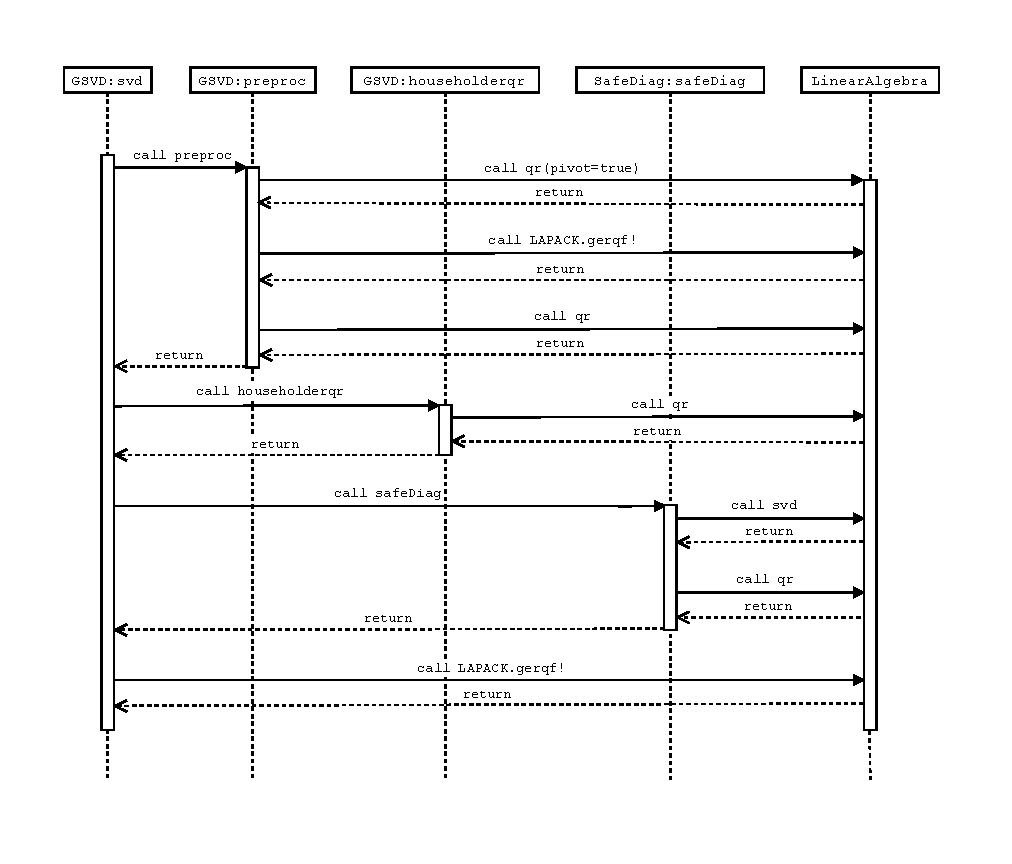
\includegraphics[width=\linewidth]{fig/gsvd_seq_diag.pdf}
              	\caption{Sequence diagram for the GSVD}
               \label{seq_diag}
        \end{figure} 


\item The details of each major functions are discussed below. 

\begin{itemize} 
\item \fbox{\texttt{GSVD:preproc}}

    This step is to reduce two input matrices $A$ and $B$ into two upper triangular forms. This is done via a call to \texttt{preproc}. This function makes use of three fundamental orthogonal decompositions. 
    \begin{enumerate}
    	\item First is QR decomposition with column pivoting to reveal the numerical rank of $B$ and $[A; B]$ without forming the matrix explicitly. This is done by a call to \texttt{qr(A, pivot=Val(true)))}. Let \texttt{tolB} as the tolerance to determine the effective rank of $B = \ell$.
		\begin{equation*}
			tol_{B} = max\{p, n\}\Vert B \Vert_1 \epsilon
		\end{equation*}
		where $\epsilon$ is the machine precision of \texttt{Float64}. \\
		We also use QR decomposition with column pivoting again on the leftmost $n-\ell$ columns of $A$. Similarly, by defining
		\begin{equation*}
			tol_{A} = max\{m, n\}\Vert A \Vert_1 \epsilon
		\end{equation*}
		we compute the effective rank of $[A; B] = k+ \ell$.
		\item Second is RQ decomposition of the top $\ell$ rows of $B$ if $n > \ell$ via a call to \texttt{LAPACK.gerqf!}. It is called a second time on $A$ if $n - \ell > k$.
		\item Third is QR decomposition of $A$ when $m > k$ by calling \texttt{qr}. 
	\end{enumerate}
	Upon return to \texttt{svd}, two of the upper triangular matrices overwrites $A$ and $B$, the orthogonal matrices are placed in U, V, and Q and rank information is stored in $k$ and $\ell$.

\item \fbox{\texttt{GSVD:householderqr}} 
    
    This step is to reduce two upper triangular matrices to one and is done by calling \texttt{householderqr}. On entry, two triangular matrices are stacked together and passed as the arguments of \texttt{qr}. On exit, $Q_1$ and $Q_2$ overwrites inputs.  
    
\item \fbox{\texttt{SafeDiag:safediag}}
    
    This step calls \texttt{safeDiag} from module \texttt{SafeDiag}. This function requires SVD, and QR decomposition. This is done by calls to \texttt{svd}, \texttt{qr} respectively. 
    \begin{enumerate}
    	\item We first compute SVD of $Q_{2}$. To preserve the order of $\{\cos\theta\}$, we have to reverse the order of the singular values of $Q_{2}$. 
		\item Since $\{\cos\theta\}$ are already sorted, we take advantage of binary search to find the threshold $r$.
		\item QR decomposition of the multiply of $Q_{1}$ and right singular vectors of $Q_{2}$. $R$ is not only triangular but diagonal. However, sanitization is necessary to assure the non-negativity of the diagonal entries. 
    \end{enumerate}
    
    It return $U_1, V_1, Z_1, C, S$ on exit.   

\item Post-processing:

    In this step, we update matrix $U$, $V$ and $Q$ by matrix-matrix multiply. To formulate $R$, we utilize RQ decomposition via a call to \texttt{LAPACK.gerqf!}. Finally, we put matrices $U, V, C, S, Q$ and $k$, $\ell$ into the constructor of \texttt{GeneralizedSVD} as return. 

\end{itemize}

\item We implement the GSVD algorithm in Julia 1.3 using \texttt{Float64} data. Our current implementation is able to be extended for {\tt Float32} type in the future. 

\end{enumerate} 


\subsection{Lessons and caveats} 
We capture some pitfalls that might be a bottleneck, 
and thus are worth mentioning.
\begin{itemize} 

\item {\bf Some inconsistent interface design.}

As a modern programming language, Julia supports multiple dispatch, that is, parametric polymorphism. A good example is that the GSVD interface reuses the name of the SVD of a single matrix $A$ by taking two matrices as arguments. Unfortunately, this principle is not fully implemented. For instance, when computing the matrix norm of {\tt [1 2 3; 4 5 6; 7 8 9]}, one may intuitively call \texttt{norm([1 2 3; 4 5 6; 7 8 9])}. However, this will not produce the desired result as shown below. What it actually computes is the 2-norm of the vector formed by iterating every entry of this matrix. Equivalently, it computes {\tt norm([1 2 3 4 5 6 7 8 9])}. To get the proper matrix norm, instead, one may want to use \texttt{opnorm([1 2 3; 4 5 6; 7 8 9])}. 

\begin{table}[H]
\centering
\begin{tabular}{|| c | c ||} \hline
Julia command/result & MATLAB command/result\\ [0.5ex] \hline\hline
\makecell{\texttt{norm([1 2 3; 4 5 6; 7 8 9])} \\
16.881943016134134} & \makecell{\texttt{norm([1 2 3;4 5 6;7 8 9])} \\ 16.8481} \\
\hline\hline
\makecell{\texttt{opnorm([1 2 3; 4 5 6; 7 8 9])} \\
16.84810335261421} & N/A \\
\hline\hline
\end{tabular}
\label{norm-api}
\end{table}

\item {Performance relies on ``proper'' implementation.}

Our GSVD algorithm involves many operations with subarrays and submatrices. Naturally, we would use {\tt [start\_i:end\_i,start\_j:end\_j]} to get a block matrix (slicing) from the entire matrix. However, in Julia, this could be a significant performance issue since slicing an array/matrix creates a copy of the selected subarray/submatrix, which is computational expensive. For instance, if we want to get the sum of subarray, we might do the following in Julia:  
%To make things worse, if a sliced matrix is passed as the return value, the result will be inaccurate as it is not overwritten in the original matrix. 
\begin{verbatim}
    x = rand(10^6);
    fcopy(x) = sum(x[2:end-1]);
    @time fcopy(x);
  	    0.003051 seconds (7 allocations: 7.630 MB)
\end{verbatim}

An alternative is to create a ``view'' of the array, which is an array object that actually references the data of the original array in-place, without making a copy. This can be done for individual slices by calling function \texttt{view}, or more simply for a whole expression or block of code by putting macro \texttt{@views} in front of that expression. This could improve the performance significantly. In the following code, we rewrite the function to calculate the sum of suarray with macro \texttt{@views}. One can tell that by doing so, the speedup is three-fold. 

%\begin{lstlisting}[language=julia, style=jlcodestyle]
\begin{verbatim}
    x = rand(10^6);
    @views fview(x) = sum(x[2:end-1]);
    @time fview(x);
        0.001020 seconds (6 allocations: 224 bytes)
\end{verbatim}
%\end{lstlisting}

\end{itemize} 

Many other features of Julian have not been studied and explored 
by the author, most notably, parallelism. This could be 
a good direction for future work. 


\subsection{GSVD in other languages}  
A number of numerical computing platforms feature 
the GSVD is listed in the following table. 
%Table \ref{tab:gsvdlang} is a list of ones we know of. 
    
%\begin{table}%[H]
%\centering
\begin{center} 
\scalebox{0.80}{
\begin{tabular}{|c|c|} \hline
Language & GSVD Documentation \\ \hline\hline
            Native Julia (proposed) &  \makecell[l]{\texttt{svd(A, B) -> GeneralizedSVD} \\ Computes the generalized SVD of \texttt{A} and \texttt{B},  returning a \texttt{GSVD} factorization\\ object \texttt{F}, such that \\ \texttt{A = F.U*F.C*F.R*F.Q'} and \texttt{B = F.V*F.S*F.R*F.Q'}.}\\ \hline
            Julia 1.3 (LAPACK wrapper) &  \makecell[l]{\texttt{svd(A, B) -> GeneralizedSVD} \\ Computes the generalized SVD of \texttt{A} and \texttt{B},  returning a \texttt{GeneralizedSVD}\\ factorization object \texttt{F}, such that \\ \texttt{A = F.U*F.D1*F.R0*F.Q'} and \texttt{B = F.V*F.D2*F.R0*F.Q'}.}\\ \hline
            MATLAB (2019b) & \makecell[l]{\texttt{[U,V,X,C,S] = gsvd(A,B)} \\
            Returns unitary matrices \texttt{U} and \texttt{V}, a (usually) square matrix \texttt{X}, and \\ nonnegative diagonal matrices \texttt{C} and \texttt{S} so that \\
                \texttt{A = U*C*X', B = V*S*X', C'*C + S'*S = I}.}\\ \hline
            Mathematica & \makecell[l]{\texttt{SingularValueDecomposition[{m,a}]} \\
            Gives a list of matrices \{\texttt{{u,ua},{w,wa},v}\} such that \texttt{m} can be written as \\ \texttt{u.w.Conjugate[Transpose[v]]} and \texttt{a} can be written as \\ \texttt{ua.wa.Conjugate[Transpose[v]]}. } \\ \hline
            R (geigen v2.3, LAPACK wrapper) & \makecell[l]{\texttt{z <- gsvd(A, B)}\\
            Computes The Generalized Singular Value Decomposition of matrices \\ $A$ and $B$ such that $A = UD_{1}[0 \ R]Q^{T}$ and $B = VD_{2}[0 R]Q^{T}$. Note that \\ the return value is the same as the output of LAPACK 3.6 and above. }
            \\\hline
            Python (R. Luo's thesis) &  \makecell[l]{Didn't disclose API design. The author defined GSVD as follows: \\
            Given two $M_i$-by-$N$ column-matched but row-independent matrices $D_{i}$, \\ each with full column rank and $N \leq Mi$, the GSVD is an exact \\ simultaneous factorization $Di = Ui \Sigma_i V^T, i = 1, 2$. $U_i$ is $M_i$-by-$N$ and \\ are column-wise orthonormal and $V$ is $N$-by-$N$ nonsingular matrix with\\ normalized rows. $diag(\Sigma_i)$ returns two lists of $N$ positive values and \\the ratios are called the generalized singular values.} \\ \hline
        \end{tabular}
} 
\end{center} 
% \caption{GSVD in different languages} \label{tab:gsvdlang}
%\end{table}
    

\newpage
    \subsection{Accuracy (backward stability)}
    \paragraph{Metric.}
    We define the following metrics in order to test backward stability:
    \begin{align} 
        res_A &= \frac{\Vert U^TAQ - CR\Vert_1}{max(m,n)\Vert A \Vert_1 \epsilon}  \\[0.8em]  \label{backward_error_1}
        res_b &= \frac{\Vert V^TBQ - SR\Vert_1}{max(p,n)\Vert B \Vert_1 \epsilon}  \\[0.8em]  
        orth_U &= \frac{\Vert I - U^TU\Vert_1}{m \epsilon} \\[0.8em]  
        orth_V &= \frac{\Vert I - V^TV\Vert_1}{p \epsilon} \\[0.8em]  
        orth_Q &= \frac{\Vert I - Q^TQ\Vert_1}{n \epsilon} \label{backward_error_5}
    \end{align}
    where $\epsilon$ is machine precision of input data type.
    
    \subsubsection{Numerical examples of small matrices}

    We also record the stability metrics computed by both versions in Julia in Table \ref{tab:sta_test_1}.
        \begin{table}[H]
        \centering
        \begin{tabular}{||c | c || c | c | c | c | c||} 
         \hline
         & Version & $res_A$ & $res_B$ & $orth_U$ & $orth_V$ & $orth_Q$ \\ [0.5ex] 
         \hline\hline
         \multirow{2}{5em}{Example 1} & proposed & 0.2956 & 0.5646 & 0.5308 & 1.0417 & 1.1790 \\ 
         & Julia 1.3 & 0.3599 & 0.4571 & 0.9117 & 1.7083 & 1.3250 \\
        \hline\hline
        \multirow{2}{5em}{Example 2} & proposed & 0.6173 & 0.4098 & 1.5000 & 0.5613 & 1.3998 \\ 
         & Julia 1.3 & 0.5068 & 0.5689 & 1.4583 & 0.9245 & 1.2483 \\
        \hline\hline
        \multirow{2}{5em}{Example 3} & proposed & 0.4181 & 0.8941 & 0.7500 & 1.3940 & 1.3277 \\ 
         & Julia 1.3 & 0.3536 & 0.5938 & 1.4791 & 1.9540 & 1.1062\\
        \hline\hline
        \multirow{2}{5em}{Example 4} & proposed & 0.3600 & 0.5900 & 0.6558 & 0.5385 & 1.4362 \\ 
         & Julia 1.3 & 0.4449 & 0.3056 & 1.3225 & 0.7205 & 1.1814 \\
        \hline\hline
        \end{tabular}
        \caption{Stability profiling for small matrices}
        \label{tab:sta_test_1}
        \end{table}
        
    \subsubsection{Random dense matrices}
        \paragraph{Test matrix generation.} As discussed in Section \ref{def}, we test stability on four cases depending on the row and column size of the input matrix pair. In this section, we test random dense matrices of \texttt{Float64}. For each case, we choose four subcases from low to high matrix size. We generate a total of 320 random matrix pairs, 20 for each subcase.
        
        \paragraph{Results.}
        As a demonstration, we list the results of five stability metrics for each subcase of a single test run in Table \ref{tab: sta_test_2}. All 320 test runs yield results no greater than two. 
    \newpage 
    
    \begin{table}[!htbp]
        \centering
        \begin{tabular}{||c | c | c | c | c || c | c | c | c | c||} 
         \hline
         & $m$ & $p$ & $n$ & $k+l$ & $res_A$ & $res_B$ & $orth_U$ & $orth_V$ & $orth_Q$ \\ [0.5ex] 
         \hline\hline
         \multirow{4}{5em}{$m \geq n$ \\ $p \geq n$} & 60 & 50 & 40 & 40 & 0.1607 & 0.2710 & 0.7924 & 1.0079 & 0.4609 \\
         & 300 & 250 & 200 & 200 & 0.0369 & 0.0484 & 0.5041 & 0.6408 & 0.3202 \\
         & 900 & 750 & 600 & 600 & 0.0181 & 0.0193 & 0.3952 & 0.5157 & 0.2307 \\
         & 1500 & 1250 & 1000 & 1000 & 0.0120 & 0.0142 & 0.3702 & 0.4129 & 0.1847 \\
        \hline\hline
         \multirow{4}{5em}{$m \geq n > p$} & 60 & 40 & 50 & 50 & 0.1529 & 0.2261 & 0.7653 & 1.1960 & 0.6074 \\
         & 300 & 200 & 250 & 250 & 0.0412 & 0.0620 & 0.5559 & 0.7492 & 0.3150 \\
         & 900 & 600 & 750 & 750 & 0.0169 & 0.0232 & 0.4174 & 0.5250 & 0.2411 \\
         & 1500 & 1000 & 1250 & 1250 & 0.0122 & 0.0160 & 0.3726 & 0.4723 & 0.2080 \\
         \hline\hline 
         \multirow{4}{5em}{$p \geq n > m$} & 40 & 60 & 50 & 50 & 0.1672 & 0.2028 & 1.1293 & 0.9373  & 0.4217\\
         & 200 & 300 & 250 & 250 & 0.0595 & 0.0530 & 0.7064 & 0.5855 &  0.3065 \\
         & 600 & 900 & 750 & 750 & 0.0231 & 0.0231 & 0.5178 & 0.4186 & 0.2112 \\
         & 1000 & 1500 & 1250 & 1250 & 0.0164 & 0.0153 & 0.4543 & 0.3673 & 0.1778 \\
         \hline \hline
         \multirow{4}{5em}{$n > m$\\ $n > p$ } & 20 & 30 & 60 & 50 & 0.0483 & 0.0464 & 0.5472 & 0.5358 & 0.4547\\
         & 200 & 300 & 600 & 500 & 0.0120 & 0.0105 & 0.3036 & 0.3030 & 0.2374 \\
         & 400 & 600 & 1200 & 1000 & 0.0081 & 0.0072 & 0.2888 & 0.2813 & 0.2315\\
         & 1000 & 1500 & 3000 & 2500 & 0.0053 & 0.0047 & 0.2700 & 0.2605 & 0.2410 \\
         \hline
        \end{tabular}
        \caption{Stability profiling for random dense matrices}
        \label{tab: sta_test_2}
        \end{table}
    
    \subsubsection{Special types of matrices}
        
    \newpage
    \subsection{Timing}
        We want to evaluate the timing performance of our implementation between current version in Julia and MATLAB. 
        
        \paragraph{vs. Julia 1.3}
        For the comparison with Julia 1.3, we also spilt into four cases. Each case, we calculated the average CPU timing of 10 runs. In all cases, we can see that the speedup is exponential when input size is greater than a few hundreds. 
        
        \begin{figure}[H]
            \centering
            \begin{minipage}{.65\textwidth}
              \centering
              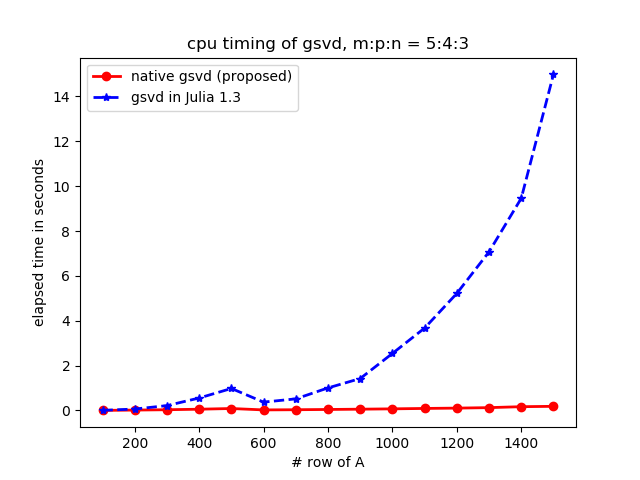
\includegraphics[width=\linewidth]{fig/m p n 5 4 3.png}
            \end{minipage}%
        \end{figure}
        
        \begin{figure}[H]
            \centering
            \begin{minipage}{.65\textwidth}
              \centering
              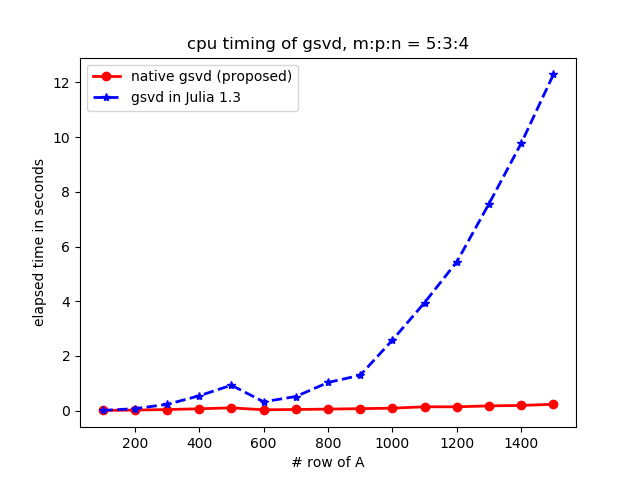
\includegraphics[width=\linewidth]{fig/m p n 5 3 4.png}
            \end{minipage}
            \label{cur_new_1}
        \end{figure}
    
        \begin{figure}[H]
            \centering
            \begin{minipage}{.65\textwidth}
              \centering
              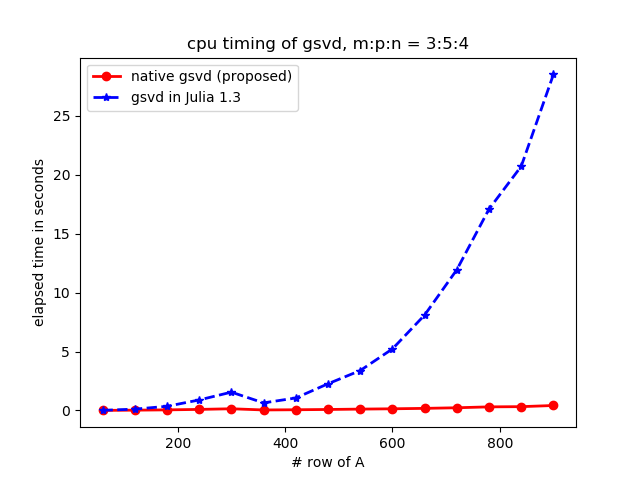
\includegraphics[width=\linewidth]{fig/m p n 3 5 4.png}
            \end{minipage}%
            
        \end{figure}
        
        \begin{figure}[H]
            \centering
            \begin{minipage}{.65\textwidth}
              \centering
              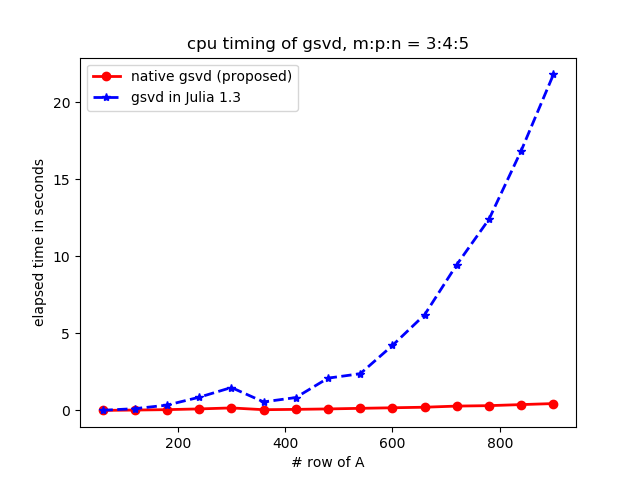
\includegraphics[width=\linewidth]{fig/m p n 3 4 5.png}
            \end{minipage}
            \label{cur_new_2}
        \end{figure}
        
        \paragraph{vs. MATLAB.}
        For the comparison with MATLAB 2019b, we specify the input as square matrix. Our implementation is still slower than MATLAB. The major reason is due to the significant difference of decomposition discussed in \ref{def} and \ref{def_mat}. 
        
        \begin{figure}[H]
            \centering
            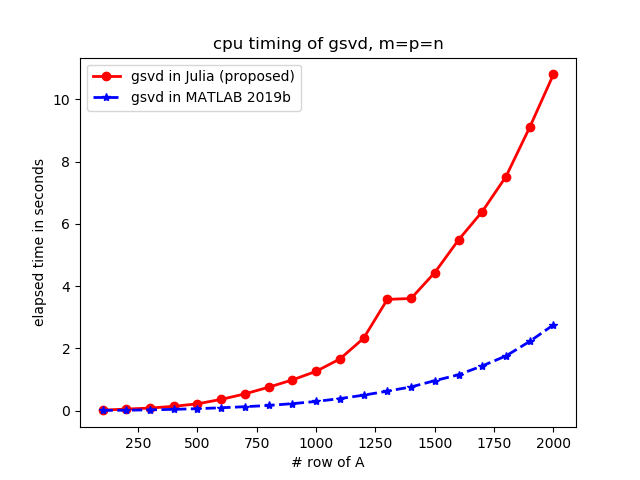
\includegraphics[width=0.65\linewidth]{fig/Julia VS MATLAB m=n=p.png}
            \label{julia_matlab}
        \end{figure}
    
    \newpage
    
    \paragraph{Profile.}
    As detailed in \ref{alg}, our algorithm insists of four parts: pre-processing, QR, CSD and post-processing. Here, we measure the CPU time spent in the first three parts and total time, denoted as $t_{pre}, t_{qr}, t_{csd}$ and   $t_{all}$ and calculated the percentages that each part spent to total time, denoted as $p_{pre}, p_{qr}, p_{csd}$. Still, we separate our test into four cases and record the average of 10 test runs. \textcolor{red}{In most cases, pre-processing dominates the computation effort}. This motivates us to explore time profiling of pre-processing. 
    
    \begin{center}
        \begin{table}[H]
        \begin{tabular}{||c | c | c | c || c | c | c | c | c | c | c ||} 
         \hline
          & $m$ & $p$ & $n$ & $t_{pre}$ & $p_{pre}$ & $t_{qr}$ & $p_{qr}$ & $t_{csd}$ & $p_{csd}$ & $t_{all}$ \\ [0.5ex] 
         \hline\hline
         \multirow{4}{5em}{$m \geq n$ \\ $p \geq n$} & 1500 & 1200 & 1000 & 0.6242 & 41.13\% & 0.1683 & 11.09\% & 0.6011 & 39.61\% & 1.5175\\
         & 500 & 500 & 500 & 0.0651 & 26.78\% &  0.0347 & 14.29\% & 0.1191 & 48.94\% & 0.2433 \\
         & 650 & 310 & 230 & 0.0418 & 54.63\% & 0.0084 & 11.08\% & 0.0195 & 25.47\% & 0.0766 \\
         & 430 & 610 & 210 & 0.0345 & 47.65\% & 0.0067 & 9.25\% & 0.0247 & 34.11\% & 0.0725 \\
        \hline\hline
         \multirow{4}{5em}{$m \geq n > p$} & 1500 & 1000 & 1200 & 1.500 & 60.09\% & 0.1815 & 7.27\% & 0.6811 & 27.28\% & 2.4963 \\ 
         & 720 & 220 & 540 & 0.1182 & 73.65\% & 0.0074 & 4.61\% & 0.0256 & 15.94\% & 0.1605 \\
         & 440 & 180 & 440 & 0.0651 & 65.84\% & 0.0053 & 5.37\% & 0.0221 & 22.41\% & 0.0989 \\
         & 370 & 290 & 350 & 0.0659 & 51.61\% & 0.0123 & 9.65\% & 0.0400 & 31.34\% & 0.1278 \\
         \hline\hline 
         \multirow{4}{5em}{$p \geq n > m$} & 1000 & 1500 & 1200 & 0.5234 & 23.23\% & 0.2789 & 12.37\% & 1.2630 & 56.06\% & 2.2529 \\
         & 250 & 300 & 300 & 0.0205 & 24.96\% & 0.0129 & 15.75\% & 0.0397 & 48.25\% & 0.0822 \\
         & 360 & 660 & 600 & 0.0645 & 18.33\% & 0.0436 & 12.39\% & 0.2103 & 59.72\% & 0.3521 \\
         & 130 & 520 & 480 & 0.0311 & 14.52\% & 0.0215 & 10.02\% & 0.1391 & 64.79\% & 0.2146 \\
         \hline \hline
         \multirow{4}{5em}{$n > m$\\ $n > p$} & 1000 & 1200 & 1500 & 1.7532 & 48.51\% & 0.2038 & 5.64\% & 1.4467 &  40.03\% & 3.6136\\
         & 260 & 600 & 770 & 0.2791 & 38.86\% & 0.0441 & 6.14\% & 0.3459 & 48.17\% & 0.7181 \\
         & 370 & 250 & 700 & 0.1385 & 86.69\% & 0 & 0\% & 0 & 0\% & 0.1598\\
         & 120 & 120 & 400 & 0.0296 & 96.70\% & 0 & 0\% & 0 & 0\% & 0.0307\\
         \hline
        \end{tabular}
        \caption{Time profiling for GSVD}
        \label{table:2}
        \end{table}
        \end{center}
        
        \newpage
    
    \paragraph{Pre-processing.}To avoid skipping steps in pre-processing, we use rank-deficient matrix as input of $B$. Likewise the time profiling of GSVD, we record absolute time spent in each part and the relative percentage to total time. The meaning of subscript in Table \ref{table:3} is explained below:
    \begin{enumerate}
        \item $qrpB$: QR decomposition with column pivoting of $B$.
        \item $genV$: Generate $V$.
        \item $updateA1st$: First time to update $A$.
        \item $genQ$: Geneate $Q$.
        \item $rqB$: RQ decomposition of $B$.
        \item $updateA2nd$: Second time to update $A$.
        \item $updateQ1st$: First time to update $Q$.
        \item $qrpA$: QR decomposition with column pivoting of $A$.
        \item $genU$: Generate $U$.
        \item $updateA3rd$: Third time to update $A$.
        \item $updateQ2nd$: Second time to update $Q$.
        \item $rqA$: RQ decomposition of $A$.
        \item $updateQ3rd$: Third time to update $Q$.
        \item $qrA$: QR decomposition of $A$.
        \item $updateU$: Update $U$.
    \end{enumerate}
    
    \newpage
    
    \begin{table}[H]
        \centering 
        \resizebox{0.8\columnwidth}{!}{%

        \begin{tabular}{||c | c | c | c ||} 
         \hline
            & \makecell{$m = 1200, p = 1000, n = 900$ \\ $l = 800, k = 100$} & \makecell{$m = 500, p = 500, n = 600$ \\ $l = 400, k = 200$} & \makecell{$m = 250, p = 200, n = 200$ \\ $l = 150, k = 50$} \\ [0.5ex]
        \hline
          $t_{qrpB}$ ($p$-by-$n$) & 0.036821 &  0.018432 & 0.002894 \\ [0.5ex] \hline
          $p_{qrpB}$ & 15.29\% &  21.59\% & 11.19\% \\ [0.5ex] \hline
          $t_{genV}$ ($p$-by-$p$) & 0.022350 &  0.006850 & 0.001578 \\ [0.5ex] \hline
          $p_{genV}$ & 9.28\% &  8.02\% & 6.10\% \\ [0.5ex] \hline
          $t_{updateA1st}$ ($m$-by-$n$) & 0.012765 & 0.005162 & 0.000736 \\ [0.5ex] \hline
          $p_{updateA1st}$ & 5.30\% & 6.05\% & 2.84\% \\ [0.5ex] \hline
          $t_{genQ}$ ($n$-by-$n$) & 0.002553 & 0.001187 & 0.000195 \\ [0.5ex] \hline
          $p_{genQ}$ & 1.06\% & 1.39\% & 0.75\% \\ [0.5ex]
        \hline\hline
        
          $t_{rqB}$ ($l$-by-$n$) & 0.024456 & 0.010305 & 0.001856 \\ [0.5ex] \hline
          $p_{rqB}$ & 10.16\% & 12.07\% & 7.18\% \\ [0.5ex] \hline
          $t_{updateA2nd}$ ($m$-by-$n$) & 0.019261 & 0.005071 & 0.000781 \\ [0.5ex]\hline
          $p_{updateA2nd}$ & 8.00\% & 5.94\% & 3.02\% \\ [0.5ex]\hline
          $t_{updateQ1st}$ ($n$-by-$n$) & 0.014279 & 0.005488 & 0.000732 \\ [0.5ex]\hline
          $p_{updateQ1st}$ & 5.93\% & 6.43\% & 2.82\% \\ [0.5ex]
         \hline\hline
         
          $t_{qrpA}$ ($m$-by-$n-l$) & 0.002878 & 0.004063 & 0.000595 \\ [0.5ex] \hline
          $p_{qrpA}$ & 1.20\% & 4.76\% & 2.30\% \\ [0.5ex] \hline
          $t_{genU}$ ($m$-by-$m$) & 0.015431 & 0.007718 & 0.001051 \\ [0.5ex]\hline
          $p_{genU}$ & 6.40\% & 9.04\% & 4.06\% \\ [0.5ex]\hline
          $t_{updateA3rd}$ ($m$-by-$l$)& 0.009105 & 0.002531 & 0.000412 \\ [0.5ex]\hline
          $p_{updateA3rd}$ & 3.78\% & 2.96\% & 1.59\% \\ [0.5ex]\hline
          $t_{updateQ2nd}$ ($n$-by-$n-l$)& 0.000289 & 0.000871 & 0.000136 \\ [0.5ex]\hline
          $p_{updateQ2nd}$ & 0.12\% & 1.02\% & 0.53\% \\ [0.5ex]\hline
          \hline
         
          $t_{rqA}$ ($k$-by-$n-l$) & 0 & 0 & 0 \\ [0.5ex] \hline
          $p_{rqA}$ & 0\% & 0\% & 0\% \\ [0.5ex] \hline
          $t_{updateQ3rd}$ ($n$-by-$n-l$)& 0 & 0 & 0 \\ [0.5ex]\hline
          $p_{updateQ3rd}$ & 0\% & 0\% & 0\% \\ [0.5ex]
          \hline\hline
          
          $t_{qrA}$ ($m-k$-by-$l$) & 0.022391 & 0.002823 & 0.001756 \\ [0.5ex] \hline
          $p_{qrA}$ & 9.30\% & 4.76\% & 6.79\% \\ [0.5ex] \hline
          $t_{updateU}$ ($m$-by-$m-k$)& 0.022113 & 0.001799 & 0.000850 \\ [0.5ex]\hline
          $p_{updateU}$ & 9.18\% & 2.11\% & 3.28\% \\ [0.5ex]
          \hline\hline
          $t_{all}$ & 0.240752 & 0.085373 & 0.025867 \\[0.5ex]
          \hline
        \end{tabular}
        }
        \caption{Time profiling for Preprocessing}
    \label{table:3}
    \end{table}


\newpage
 

\subsection{Genomic signal processing}
The GSVD is applicable for comparative analysis of genome-scale expression datasets of two different organisms \cite{alter2003generalized} and is further extended to tensor \cite{sankaranarayanan2015tensor}.

\subsection{Tikhonov regularization}
Tikhonov regularization in general form can be analyzed with the truncated GSVD when we are to solve the ill-posed linear least squares problem. \cite{hansen1989regularization} \cite{dykes2014simplified} \cite{wei2016tikhonov} Computerized ionospheric tomography \cite{bhuyan2004application} is one of the applications in this regard. 

\subsection{Matrix pencil $A - \lambda B$}
The GSVD is also used in the field of the canonical structure of matrix pencil $A-\lambda B$. \cite{kaagstrom1984generalized} More specifically, the column and row nullities of $A$ and $B$ and common null space reveal the information about the Kronecker structure of $A-\lambda B$.

\subsection{Generalized total least squares problem}
By making use of the GSVD, one can solve the generalized TLS problem. TLS is also called error-in-variable regression in statistics domain. The great advantage of the GSVD is that it replaces these implicit transformation of data procedures by one, which is numerically reliable and can more easily handle (nearly) singular associated error covariance matrix. \cite{van1989analysis} \cite{bai1992csd}

\subsection{Oriented energy and oriented signal-to-signal ratio}
In the context of oriented energy, one of the concerns is to characterize the signal-to-signal ratio of two given sequences of $m$-vectors $\{a_k\}$, $\{b_k\}$, $k = 1,\cdots,n$ with associated $m$-by-$n$ matrices $A$ and $B$. \cite{de1988mathematical} In other words, we're primarily interested in how to separate the desired signal (for instance $\{a_k\}$) from the undesired one ($\{b_k\}$). More specifically, given that rank($B$) = $l$, the question transforms to find the optimal $l$-dimensional subspace where the desired signal sequence $\{a_k\}$ can be optimally distinguished from the corrupting sequence $\{b_k\}$.

\subsection{Subspaces of the $U$ matrix}\cite{edelman2019gsvd}
The $U$ matrix of the GSVD provides orthonormal bases for three mutually orthogonal subspaces that are powerful in many applications: 

\begin{equation*}
    U = \begin{bmatrix}
        \makecell{U_{1} = \\ \text{orthogonal basis for} \\ \{Ax:Bx=0\}} & \makecell{U_{2} = \\ \text{completion to all of} \\ col(A)=\{Ax\}} & \makecell{U_{3} = \\ \text{orthonomal basis for} \\ col(A)^{\perp}}
    \end{bmatrix}
\end{equation*}
The ``completion'' referred to in the above equation means that taken together, the columns of $U_1$ and $U_2$ form and orthonormal basis for $col(A)$.

\subsubsection{Linear discriminant analysis}
Howland and Park \cite{howland2003structure} \cite{kim2005dimension} applied the GSVD to discriminant analysis to overcome the limitation of nonsingular covariance matrices that are used to represent the scatter within and between clusted text data. 

\subsubsection{One Way ANOVA (Analysis of variance)}
A commonly used statistics test is to decide whether a proposed clustering of a vector $v$ is justified. The test takes the average square component in the $U_2$ direction and divides it by the average square component in the $U_3$ direction. \cite{wikipedia_2020}

\subsection{The Jacobi ensemble from random matrix theory is a GSVD}\cite{edelman2019gsvd}
Classical random matrix theory centers are Hermite, Laguerre, and Jacobi ensembles. Historically, they are presented in eigenvalue format, but we have argued that the eigenvalue, SVD, GSVD formats, respectively, are mathematically more natural providing simpler derviations and clearer insights. 

\newpage
\bibliographystyle{plain} 
\bibliography{ref}

\end{document}
